\setcounter{section}{2}
\section{TÍNH CHẤT CỦA PHÉP KHAI PHƯƠNG}
\subsection{Trọng tâm kiến thức}
\begin{tomtat}
\subsubsection{Căn thức bậc hai của một bình phương}
\begin{boxdn}
	\begin{itemize}
	\item
	Với mọi số thực $a$, ta có $\sqrt{a^{2}}=|a|$.
	\item
	Với biểu thức $A$ bất kì, ta có $\sqrt{A^{2}}=|A|$, nghĩa là 
	\begin{itemize}
	\item $\sqrt{A^{2}}=A$ khi $A \geq 0$ (tức là khi $A$ nhận giá tri không âm); 
	\item $\sqrt{A^{2}}=-A$ khi $A<0$ (tức là khi $A$ nhận giá trị âm).
	\end{itemize}
	\end{itemize}
\end{boxdn}
\subsubsection{Căn thức bậc hai của một tích}
\begin{boxdn}
	\begin{itemize}
	\item 
	Với hai số thực $a$ và $b$ không âm, ta có
	$
	\sqrt{a\cdot b}=\sqrt{a} \cdot \sqrt{b}.
	$
	\item
	Với hai biểu thức $A$ và $B$ nhận giá trị không âm, ta có
	$
	\sqrt{A \cdot B}=\sqrt{A} \cdot \sqrt{B}.
	$
	\end{itemize}
\end{boxdn}
\begin{nx}%Nhận xét: 
	Như hai ví dụ trên, tuỳ từng trường hợp mà ta biến đổi $\sqrt{ab}=\sqrt{a} \cdot \sqrt{b}$ hoặc $\sqrt{a} \cdot \sqrt{b}=\sqrt{ab}$ $(a \geq 0$ và $b \geq 0)$ để việc tính toán trở nên dễ dàng hơn.
\end{nx}
\begin{boxdn}
	Với số thực $a$ bất kì và $b$ không âm, ta có
	$
	\sqrt{a^{2} b}=|a| \sqrt{b}.
	$
	Biến đổi này được gọi là {\it đưa thừa số ra ngoài dấu căn}.
	Ngược lại, ta có biến đổi {\it đưa thừa số vào trong dấu căn}:	
	\begin{enumEX}[\itemCI]{2}
	\item Nếu $a \geq 0$ thì $a \sqrt{b}=\sqrt{a^{2} b}$;
	\item Nếu $a<0$ thì $a \sqrt{b}=-\sqrt{a^{2} b}$.
	\end{enumEX}	
\end{boxdn} %Nhận xét: 
\begin{nx}
	Tổng quát hơn, với biểu thức $A$, $B$ mà $B \geq 0$, ta có $\sqrt{A^{2} B}=|\mathrm{A}| \sqrt{B}$.
\end{nx}
\subsubsection{Căn thức bậc hai cùa một thương}
\begin{boxdn}
	\begin{itemize}
	\item
	Với số thực $a$ không âm và số thực $b$ dương, ta có
	$
	\sqrt{\dfrac{a}{b}}=\dfrac{\sqrt{a}}{\sqrt{b}}.
	$
	\item
	Với biểu thức $A$ nhận giá trị không âm và biểu thức $B$ nhận gia tri dương, ta có
	$
	\sqrt{\dfrac{A}{B}}=\dfrac{\sqrt{A}}{\sqrt{B}}.
	$
	\end{itemize}
\end{boxdn}
\begin{nx} %Nhân xét: 
	Tuỳ từng trường hợp mà ta biến đổi \begin{center}
	$\sqrt{\dfrac{a}{b}}=\dfrac{\sqrt{a}}{\sqrt{b}}$ hoặc $\dfrac{\sqrt{a}}{\sqrt{b}}=\sqrt{\dfrac{a}{b}}$ ($a \geq 0$ và $b>0$)
	\end{center} để việc tính toán trở nên dễ dàng hơn.
\end{nx}
\end{tomtat}
%%%%%%%%%%%%%%
\subsection{Các dạng bài tập}
%----------------
\begin{dang}{Tính toán, rút gọn biểu thức dạng $\sqrt{A^2}$}
	Vận dụng hằng đẳng thức $\sqrt{A^2} = \left|A\right| = \heva{A &\text{ nếu } A \ge 0 \\ -A &\text{ nếu } A<0.}$
\end{dang}
%%==========Ví dụ 11
\begin{vd}
	Tính giá trị của các biểu thức
	\begin{listEX}[4]
	\item $\sqrt{6^2}$;
	\item $\sqrt{(-5)^2}$;
	\item $\sqrt{16^{2}}$;
	\item $(\sqrt{12})^{2}$;
	\item $(-\sqrt{0{,}36})^{2}$;
	\item $(\sqrt{5})^{2}+(-\sqrt{1{,}21})^{2}$;
	\item $\sqrt{\left(-3\right)^2}+3$;
	\item $(-\sqrt{9})^{2}+\sqrt{(-9)^{2}}$.
	\end{listEX}
	\loigiai{
	\begin{listEX}[1]
	\item $\sqrt{6^2}=\big|6\big|=6$.
	\item $\sqrt{(-5)^2}=\big|5\big|=5$.
	\item $\sqrt{16^{2}}=|16|=16$.
	\item $(\sqrt{12})^{2}=12$.
	\item $(-\sqrt{0{,}36})^{2}=0{,}36$.
	\item $(\sqrt{5})^{2}+(-\sqrt{1{,}21})^{2}=5+1{,}21=6{,}21$.
	\item Ta có $\sqrt{(-3)^2}=|-3|=3$ nên $\sqrt{(-3)^2}+3=3+3=6$.
	\item $(-\sqrt{9})^{2}+\sqrt{(-9)^{2}}=9+|-9|=9+9=18$.
	\end{listEX}
	}
\end{vd}
%%==========Ví dụ 12
\begin{vd} %vi du 2. 
	Rút gọn các biểu thức sau:
	\begin{enumEX}{3}
	\item $\sqrt{(1-\sqrt{2})^{2}}$;
	\item $\sqrt{(a-\sqrt{5})^{2}}$ với $a>3$;
	\item $\sqrt{a^{6}}$ với $a<0$.
	\end{enumEX}
	\loigiai{
	\begin{enumEX}{1}
	\item $\sqrt{(1-\sqrt{2})^{2}}=|1-\sqrt{2}|=\sqrt{2}-1$ (vì $1-\sqrt{2}<0$);
	\item $\sqrt{(a-\sqrt{5})^{2}}=|a-\sqrt{5}|=a-\sqrt{5}$ (vì $a-\sqrt{5}>0$ với $a>3$ );
	\item $\sqrt{a^{6}}=\sqrt{\left(a^{3}\right)^{2}}=\left|a^{3}\right|=-a^{3}$ (vì $a^{3}<0$ với $a<0)$.
	\end{enumEX}
	}
\end{vd}
%%==========Ví dụ 13
\begin{vd}
	Không sử dụng MTCT, tính:
	\begin{listEX}[2]
	\item $\sqrt{16}+(\sqrt{8})^{2}+(-\sqrt{0{,}16})^{2}$;
	\item $\sqrt{5}-\sqrt{(\sqrt{5}-1)^2}$;
	\item $1-\sqrt{2}+\sqrt{\left(1+\sqrt{2}\right)^2}$;
	\item $\sqrt{3 - 2\sqrt{2}} - \sqrt{6 - 4\sqrt{2}}$.
	\end{listEX}
	\loigiai
	{
	\begin{enumerate}
	\item $\sqrt{16}+(\sqrt{8})^{2}+(-\sqrt{0{,}16})^{2}=\sqrt{4^{2}}+8+0{,}16=4+8+0{,}16=12{,}16$.
	\item $\sqrt{5}-\sqrt{(\sqrt{5}-1)^2}=\sqrt{5}-\big|\sqrt{5}-1\big|=\sqrt{5}-\sqrt{5}+1=1$.
	\item Ta có $\sqrt{(1+\sqrt{2})^2}=|1+\sqrt{2}|=1+\sqrt{2}$ nên $1-\sqrt{2}+\sqrt{(1+\sqrt{2})^2}=1-\sqrt{2}+(1+\sqrt{2})=2$.
	\item $\sqrt{3 - 2\sqrt{2}} - \sqrt{6 - 4\sqrt{2}}=\sqrt{(\sqrt{2} - 1)^2} - \sqrt{(2 - \sqrt{2})^2}= |\sqrt{2} - 1 | - | 2 - \sqrt{2}| =\sqrt{2} - 1 - \left(2 - \sqrt{2}\right) = 2\sqrt{2} - 3$
	\end{enumerate}	
	}
\end{vd}
%%==========Ví dụ 14
\begin{vd}%[9D1B3]
	Tính giá trị của các biểu thức sau:
	\begin{listEX}[3]
	\item $\sqrt{4+2 \sqrt{3}}$; 
	\item $\sqrt{8-2 \sqrt{15}}$;
	\item $\sqrt{9-4 \sqrt{5}}$.
	\end{listEX}
	\loigiai{
	\begin{enumerate}
	\item $\sqrt{4+2 \sqrt{3}}=\sqrt{3+2 \cdot \sqrt{3}\cdot 1+1}=\sqrt{\left(\sqrt{3}+1\right)^2}=\sqrt{3}+1$;
	\item $\sqrt{8-2 \sqrt{15}}=\sqrt{5-2 \cdot \sqrt{5} \cdot \sqrt{3}+3}=\sqrt{\left(\sqrt{5}-\sqrt{3}\right)^2}=\sqrt{5}-\sqrt{3}$;
	\item $\sqrt{9-4 \sqrt{5}}=\sqrt{5-2\cdot 2 \cdot \sqrt{5}+4}=\sqrt{\left(\sqrt{5}-2\right)^2}=\sqrt{5}-2$. 
	\end{enumerate}
	} 
\end{vd}
%%==========Ví dụ 15
\begin{vd}%[9D1K2]
	Rút gọn các biểu thức 
	\begin{listEX}[2]
	\item $A =\sqrt{x^4} + \sqrt{x^6}$;
	\item $B =\sqrt{x^2 - x + \dfrac{1}{4}}$.
	\end{listEX}	
	\loigiai{
	\begin{listEX}
	\item
	Ta có $B =\sqrt{x^4} + \sqrt{x^6}=\left| x^2\right| + \left| x^3\right| = x^2 + \left| x^3\right|=\begin{cases}
	{x^2+x^3\;\text{nếu}\;x\geq 0}\\
	{ x^2-x^3\;\text{nếu}\; x < 0.}
	\end{cases}$.
	\item
	Ta có $A =\sqrt{x^2 - x + \dfrac{1}{4}}=\sqrt{\left(x - \dfrac{1}{2}\right)^2}=\left| x - \dfrac{1}{2}\right|$.\\
	Nếu $x\geq\dfrac{1}{2}$ thì $A = x - \dfrac{1}{2}$.\\
	Nếu $x<\dfrac{1}{2}$ thì $A = \dfrac{1}{2}-x$.
	\end{listEX}
	}
\end{vd}
%%==========Ví dụ 16
\begin{vd}
	Rút gọn các biểu thức sau:
	\begin{listEX}[2]
	\item $\sqrt{1-2 x+x^2}$ với $x>2$;
	\item $\left(\sqrt{1-x}\right)^2$ với $x<0$.
	\end{listEX}
	\loigiai
	{
	\begin{enumerate}
	\item Ta có $\sqrt{1-2 x+x^2}=\sqrt{(1-x)^2}=|1-x|$.\\
	Do giả thiết $x>2$ suy ra $1-x<0$ nên $|1-x|=-(1-x)=x-1$. Vì vậy
	$$
	\sqrt{1-2 x+x^2}=\sqrt{(1-x)^2}=x-1 \text { với } x>2.
	$$
	\item Từ giả thiết $x<0$ suy ra $1-x>0$. Do đó
	$
	\left(\sqrt{1-x}\right)^2=1-x.
	$
	\end{enumerate}	
	}
\end{vd}
%%==========Ví dụ 17
\begin{vd}
	\begin{enumerate}
	\item Rút gọn biểu thức $x \sqrt{x^6} \quad(x<0)$.
	\item Rút gọn và tính giá trị của biểu thức $x+\sqrt{4 x^2-4 x+1}$ tại $x=-2,5$.
	\end{enumerate}
	\loigiai
	{
	\begin{enumerate}
	\item Ta có \allowdisplaybreaks
	\begin{eqnarray*}
	x\sqrt{x^6}=x\sqrt{\left(x^3\right)^2}=x\big|x^3\big|=x\cdot \left(-x^3\right)=-x^4\;\left(\text{vì }x<0\right)
	\end{eqnarray*}
	\item Ta có \allowdisplaybreaks
	\begin{eqnarray*}
	&&x+\sqrt{4 x^2-4 x+1}\\
	&=& x+\sqrt{\left(2x-1\right)^2}\\
	&=& x+\big|2x-1\big|.
	\end{eqnarray*}
	Thay $x=-2{,}5$ vào ta có $2{,}5+\big|2\cdot 2{,}5-1\big|=\dfrac{5}{2}+4=\dfrac{13}{2}$.
	\end{enumerate}
	}
\end{vd}
%%==========Ví dụ 18
\begin{vd}%[9D1K2]
	Cho biểu thức: $P = 3x - \sqrt{x^2 - 10x + 25}$.
	\begin{listEX}[2]
	\item Rút gọn biểu thức $P$;
	\item Tính giá trị của $P$ khi $x=2$.
	\end{listEX}
	\loigiai{\begin{enumerate}
	\item $P = 3x - \sqrt{x^2 - 10x + 25}= 3x - \sqrt{(x - 5)^2}= 3x - | x - 5 |$.
	\begin{itemize}
	\item Nếu $x\geq 5$ thì $P = 3x - (x - 5) = 2x + 5$.
	\item Nếu $x<5$ thì $P = 3x + (x - 5) = 4x - 5$.
	\end{itemize}
	\item Khi $x=2<5$ thì giá trị của $P$ là $P=4\cdot 2-5=3$.
	\end{enumerate}}
\end{vd}
%%==========Ví dụ 19
\begin{vd}%[9D1K2]
	Cho biểu thức: $Q = 2x - \sqrt{x^2 + 2x + 1}$.
	\begin{listEX}[2]
	\item Rút gọn biểu thức $Q$;
	\item Tính giá trị của $x$ khi $Q=7$.
	\end{listEX}
	\loigiai{\begin{enumerate}
	\item $Q = 2x - \sqrt{x^2 + 2x + 1}= 2x - \sqrt{(x + 1)^2}= 2x - | x + 1 |$.
	\begin{itemize}
	\item Nếu $x\geq -1$ thì $Q = 2x - (x + 1) = x - 1$.
	\item Nếu $x<-1$ thì $Q = 2x + (x + 1) = 3x + 1$.
	\end{itemize}
	\item Ta phải xét hai trường hợp:
	\begin{itemize}
	\item $Q = 7\Rightarrow x - 1 = 7\Rightarrow x = 8$ (thỏa mãn $x\geq -1$).
	\item $Q = 7\Rightarrow 3x + 1 = 7\Rightarrow x = 2$ (không thỏa mãn $x<-1$).
	\end{itemize}
	Vậy $Q=7$ khi $x=8$.
	\end{enumerate}}
\end{vd}
%%==========Ví dụ 20
\begin{vd}%[9D1K3]
	Rút gọn các biểu thức sau:
	\begin{listEX}[2]
	\item $\sqrt{x+2 \sqrt{x-1}}$; 
	\item $\sqrt{x+2-2 \sqrt{x+1}}$. 
	\end{listEX}
	\loigiai{
	\begin{enumerate}
	\item $\begin{aligned}[t] 
	\sqrt{x+2 \sqrt{x-1}}&=\sqrt{x-1+2 \sqrt{x-1}+1} \\ 
	&=\sqrt{(\sqrt{x-1}+1)^2}=\sqrt{x-1}+1 \text{ (ĐK: }x\geq 1 \text{).}
	\end{aligned}$
	\item $\begin{aligned}[t] 
	\sqrt{x+2-2 \sqrt{x+1}} & =\sqrt{x+1-2 \sqrt{x+1}+1} \\ 
	&=\sqrt{\left(\sqrt{x+1}-1\right)^2}=| \sqrt{x+1}-1 | \text{ (ĐK: }x\geq -1 \text{).}
	\end{aligned}$ \\
	Nếu $x\geq 0$ thì $| \sqrt{x+1}-1 |=\sqrt{x+1}-1$. \\
	Nếu $x<0$ thì $| \sqrt{x+1}-1 |=1-\sqrt{x+1}$. 
	\end{enumerate}
	}
\end{vd}
%============
\begin{dang}{Khai căn một tích}
\end{dang}
%%==========Ví dụ 1
\begin{vd}
	Áp dụng quy tắc về căn bậc hai của một tích, hãy tính:
	\begin{listEX}[4]
	\item $\sqrt{81 \cdot 49}$;
	\item $\sqrt{25 \cdot 121}$;
	\item $\sqrt{2^2 \cdot 3^2 \cdot 5^2}$;
	\item $\sqrt{25 \cdot 1{,}21}$;
	\item $\sqrt{360 \cdot 90}$;
	\item $\sqrt{0{,}16\cdot 64}$;
	\item $\sqrt{8{,}1 \cdot 10^{3}}$;
	\item $\sqrt{12,1\cdot 160}$.
	\end{listEX}
	\loigiai{
	\begin{enumerate}
	\item $\sqrt{81 \cdot 49}=\sqrt{81} \cdot \sqrt{49}=9 \cdot 7=63$.
	\item $\sqrt{25 \cdot 121}=\sqrt{25}\cdot \sqrt{121}=5\cdot 11=55$.
	\item $\sqrt{2^2 \cdot 3^2 \cdot 5^2}=\sqrt{2^2} \cdot \sqrt{3^2} \cdot \sqrt{5^2}=2 \cdot 3 \cdot 5=30.$
	\item $\sqrt{25 \cdot 1{,}21}=\sqrt{25} \cdot \sqrt{1{,}21}=5 \cdot 1{,}1=5{,}5$;
	\item $\sqrt{360 \cdot 90}=\sqrt{36 \cdot 9 \cdot 100}=\sqrt{36} \cdot \sqrt{9} \cdot \sqrt{100}=6 \cdot 3 \cdot 10=180$.
	\item $\sqrt{0{,}16\cdot 64}=\sqrt{0{,}16} \cdot \sqrt{ 64} = 0{,}4 \cdot 8 = 3{,}2$.
	\item $\sqrt{8{,}1 \cdot 10^{3}}= \sqrt{8{,}1 \cdot 10^{2}\cdot 10} =\sqrt{81 \cdot 10^{2}} = \sqrt{81} \cdot \sqrt{10^{2}} = 9\cdot 10=90$.
	\item $\sqrt{12,1\cdot 160}=\sqrt{121\cdot 16}=\sqrt{121} \cdot \sqrt{16}=11\cdot 4=44$.
	\end{enumerate}
	}
\end{vd}
%%==========Ví dụ 2
\begin{vd}%[9D1B3]
	Áp dụng quy tắc về căn bậc hai của một tích, hãy tính:
	\begin{listEX}[4]
	\item $\sqrt{2500\cdot 4,9\cdot 0,9}$;
	\item $\sqrt{12 \cdot 250 \cdot 1,2}$;
	\item $\sqrt{41^2-40^2}$ ;
	\item $\sqrt{81\cdot 6,25-2,25\cdot 81}$.
	\end{listEX}
	\loigiai{
	\begin{enumerate}
	\item $\sqrt{2500\cdot 4,9\cdot 0,9}=\sqrt{25\cdot 49\cdot 9}=\sqrt{25} \cdot \sqrt{49} \cdot \sqrt{9}=5\cdot 7\cdot 3=105$.
	\item $\sqrt{12 \cdot 250 \cdot 1,2}= \sqrt{12 \cdot 25 \cdot 12} =\sqrt{12^2 \cdot 5^2}=\sqrt{12^2} \cdot \sqrt{5^2} =12\cdot 5 =60$;
	\item $\sqrt{41^2-40^2}=\sqrt{(41-40)\cdot (41+40)}=\sqrt{1\cdot 81}=1\cdot 9=9$;
	\item $\sqrt{81\cdot 6,25-2,25\cdot 81}=\sqrt{81\cdot (6,25-2,25)}=\sqrt{81}. \sqrt{4}=9\cdot 2=18$. 
	\end{enumerate}
	}
\end{vd}
%%==========Ví dụ 3
\begin{vd}
	\begin{listEX}[1]
	\item Tính nhanh $\sqrt{25 \cdot 49}$.
	\item Phân tích thành nhân tử $\sqrt{a b}-4 \sqrt{a}$ (với $a \geq 0, b \geq 0$).
	\end{listEX}
	\loigiai{
	\begin{listEX}[1]
	\item Ta có $\sqrt{25 \cdot 49} = \sqrt{5^2 \cdot 7^2} = \sqrt{5^2} \cdot \sqrt{7^2} = 5 \cdot 7 = 35$.
	\item Theo giả thiết $a \geq 0$; $b \geq 0$, do đó ta có
	\[\sqrt{a b}-4 \sqrt{a} =\sqrt{a}(\sqrt{b} - 4).\]	
	\end{listEX}}
\end{vd}
%%==========Ví dụ 4
\begin{vd} %Vi du 5.
	Rút gọn các biểu thức sau:
	\begin{enumEX}{3}
	\item $\sqrt{8 a \cdot 5 ab \cdot 10 b^{3}}$;
	\item $\sqrt{18(2-a)^{2}}$ với $a>2$;
	\item $\sqrt{25 a^2 b^2}$ (với $a \geq 0$; $b<0$).
	\end{enumEX}
	\loigiai{
	\begin{enumEX}{1}
	\item $\sqrt{8 a \cdot 5 ab \cdot 10 b^{3}}=\sqrt{8 \cdot 5 \cdot 10 \cdot a^{2} b^{4}}=\sqrt{400} \cdot \sqrt{a^{2}} \cdot \sqrt{\left(b^{2}\right)^{2}}=20|a| b^{2}$.
	\item 
	$\begin{aligned}[t]
	\sqrt{18(2-a)^{2}}& =\sqrt{2\cdot 9\cdot (2-a)^{2}}=\sqrt{2}\cdot \sqrt{9}\cdot \sqrt{(2-a)^{2}}
	=\sqrt{2}\cdot 3\cdot |2-a|= 3\sqrt{2}(a-2) \, (\text{vì } a>2).
	\end{aligned}$	
	\item Theo giả thiết $a \geq 0$; $b<0$, do đó
	\[\sqrt{25 a^2 b^2}=\sqrt{5^2 \cdot a^2 \cdot(-b)^2}=\sqrt{5^2} \cdot \sqrt{a^2} \cdot \sqrt{(-b)^2}=5 \cdot a \cdot(-b)=-5 a b.\]	
	\end{enumEX}
	}
\end{vd}
%=================
\begin{dang}{Nhân các căn bậc hai}
\end{dang}
%%==========Ví dụ 5
\begin{vd}
	Áp dụng quy tắc về căn bậc hai của một tích, hãy tính:
	\begin{listEX}[3]
	\item $\sqrt{5} \cdot \sqrt{20}$;
	\item $\sqrt{2} \cdot \sqrt{\dfrac{9}{8}}$;
	\item $\sqrt{72} \cdot \sqrt{50}$; 
	\item $\sqrt{12,8} \cdot \sqrt{0,2}$;
	\item $\sqrt{27} \cdot \sqrt{3}$;
	\item Tính $\sqrt{3} \cdot \sqrt{75}$.
	\end{listEX}
	\loigiai{
	\begin{enumerate}
	\item $\sqrt{5} \cdot \sqrt{20}=\sqrt{5 \cdot 20}=\sqrt{100}=10$.	
	\item $\sqrt{2} \cdot \sqrt{\dfrac{9}{8}}=\sqrt{2\cdot \dfrac{9}{8}}=\sqrt{\dfrac{9}{4}}=\dfrac{3}{2}$.	
	\item $\sqrt{72} \cdot \sqrt{50}=\sqrt{72\cdot 50}=\sqrt{36\cdot 100}=6\cdot 10=60$;
	\item $\sqrt{12,8} \cdot \sqrt{0,2}=\sqrt{12,8\cdot 0,2}=\sqrt{128\cdot 0,02}=\sqrt{64\cdot 0,04}=8\cdot 0,2=1,6$. 
	\item $\sqrt{27} \cdot \sqrt{3}=\sqrt{27 \cdot 3}=\sqrt{81}=9$.
	\item $\sqrt{3} \cdot \sqrt{75} = \sqrt{3 \cdot 75} = \sqrt{3^2 \cdot 5^2} = |3 \cdot 5| = 15$.	
	\end{enumerate}
	}
\end{vd}
%%==========Ví dụ 6
\begin{vd} %Vi du 4.
	Áp dụng quy tắc về căn bậc hai của một tích, hãy tính:
	\begin{enumEX}{3}
	\item $\sqrt{1{,}3}\cdot\sqrt{10}\cdot\sqrt{13}$.
	\item $\sqrt{10} \cdot \sqrt{5{,}2} \cdot \sqrt{52}$.	
	\item $\sqrt{4{,}9} \cdot \sqrt{30} \cdot \sqrt{12}$;
	\item $\sqrt{2{,}8} \cdot \sqrt{7} \cdot \sqrt{10}$;
	\item $\sqrt{40} \cdot \sqrt{20} \cdot \sqrt{4,5}$;
	\item $\sqrt{\dfrac{2}{3}} \cdot \sqrt{\dfrac{12}{25}} \cdot \sqrt{\dfrac{1}{2}}$. 
	\end{enumEX}
	\loigiai{
	\begin{enumEX}{1}
	\item $\sqrt{1{,}3} \cdot \sqrt{10} \cdot \sqrt{13}=\sqrt{1{,}3 \cdot 10 \cdot 13}=\sqrt{13 \cdot 13}=13$.
	\item $\sqrt{10} \cdot \sqrt{5{,}2} \cdot \sqrt{52}=\sqrt{10\cdot5{,}2\cdot 52}=\sqrt{52\cdot52}=\sqrt{52^2}=52$.
	\item $\sqrt{4,9} \cdot \sqrt{30} \cdot \sqrt{12}=\sqrt{4,9 \cdot 30 \cdot 12} = \sqrt{7^2 \cdot 3^2 \cdot 2^2}=\sqrt{7^2} \cdot \sqrt{3^2} \cdot \sqrt{2^2} = 7\cdot 3 \cdot 2 = 42$.
	\item $\sqrt{2,8} \cdot \sqrt{7} \cdot \sqrt{10}=\sqrt{2,8 \cdot 7 \cdot 10}=\sqrt{28 \cdot 7}=\sqrt{4 \cdot 7 \cdot 7}=\sqrt{2^{2} \cdot 7^{2}}=\sqrt{14^{2}}=14$.
	\item $\sqrt{40} \cdot \sqrt{20} \cdot \sqrt{4,5}=\sqrt{40\cdot 20\cdot 4,5}=\sqrt{400\cdot 9}=20\cdot 3=60$;
	\item $\sqrt{\dfrac{2}{3}} \cdot \sqrt{\dfrac{12}{25}} \cdot \sqrt{\dfrac{1}{2}}=\sqrt{\dfrac{2}{3} \cdot \dfrac{12}{25} \cdot \dfrac{1}{2}}=\sqrt{\dfrac{4}{25}}=\dfrac{2}{5}$.
	\end{enumEX}
	}
\end{vd}
%%==========Ví dụ 7
\begin{vd}%[9D1B3]
	Thực hiện các phép tính: 
	\begin{listEX}[2]
	\item $\sqrt{5}\cdot (\sqrt{125}+\sqrt{5})$;
	\item $\left(\sqrt{20}+\sqrt{45}-\sqrt{5}\right) \cdot \sqrt{5}$; 
	\item $\left(\sqrt{12}+\sqrt{3}\right) \cdot \left(\sqrt{27}-\sqrt{3}\right)$; 
	\item $\left(\sqrt{5}-\sqrt{3}+1\right)\cdot \left(\sqrt{5}-1\right)$. 
	\end{listEX}
	\loigiai{
	\begin{enumerate}
	\item Ta có $\sqrt{5}\cdot (\sqrt{125}+\sqrt{5})=\sqrt{5} \cdot \sqrt{125}+\sqrt{5} \cdot \sqrt{5}=\sqrt{5 \cdot 125}+\sqrt{25}=25+5=30$.
	\item $\left(\sqrt{20}+\sqrt{45}-\sqrt{5}\right) \cdot \sqrt{5}=\sqrt{100}+\sqrt{225}-\sqrt{25}=10+15-5=20$;
	\item $\left(\sqrt{12}+\sqrt{3}\right)\cdot \left(\sqrt{27}-\sqrt{3}\right)=\sqrt{324}-\sqrt{36}+\sqrt{81}-\sqrt{9}=18-6+9-3=18$;
	\item $\left(\sqrt{5}-\sqrt{3}+1\right)\cdot \left(\sqrt{5}-1\right)=5-\sqrt{5}-\sqrt{15}+\sqrt{3}+\sqrt{5}-1=4-\sqrt{15}+\sqrt{3}$. 
	\end{enumerate}
	}
\end{vd}
%%==========Ví dụ 8
\begin{vd}%[9D1K3]
	Thực hiện các phép tính:
	\begin{listEX}[3]
	\item $\left(\sqrt{7}+\sqrt{3}\right)^2$;
	\item $\left(\sqrt{8}-\sqrt{2}\right)^2$;
	\item $\left(5 \sqrt{3}-2 \sqrt{7}\right)\cdot \left(5 \sqrt{3}+2 \sqrt{7}\right)$. 
	\end{listEX}
	\loigiai{
	\begin{enumerate}
	\item $\left(\sqrt{7}+\sqrt{3}\right)^2=\left(\sqrt{7}\right)^2+2 \cdot \sqrt{7} \cdot \sqrt{3}+\left(\sqrt{3}\right)^2=7+2 \sqrt{21}+3=10+2 \sqrt{21}$;
	\item $\left(\sqrt{8}-\sqrt{2}\right)^2=\left(\sqrt{8}\right)^2-2 \cdot \sqrt{8} \cdot \sqrt{2}+\left(\sqrt{2}\right)^2=8-2 \sqrt{16}+2=2$;
	\item $\left(5 \sqrt{3}-2 \sqrt{7}\right)\cdot \left(5 \sqrt{3}+2 \sqrt{7}\right)=\left(5 \sqrt{3}\right)^2-\left(2 \sqrt{7}\right)^2=25\cdot 3-4\cdot 7=47$. 
	\end{enumerate}
	}
\end{vd}
%%==========Ví dụ 9
\begin{vd}%[9D1B3]
	Rút gọn biểu thức $(\sqrt{14}+\sqrt{6}) \sqrt{5-\sqrt{21}}$.
	\loigiai{
	Ta có \allowdisplaybreaks $\begin{aligned}[t] 
	\left(\sqrt{14}+\sqrt{6}\right) \sqrt{5-\sqrt{21}}&=\sqrt{2}\left(\sqrt{7}+\sqrt{3}\right) \sqrt{5-\sqrt{21}} \\ 
	&=\left(\sqrt{7}+\sqrt{3}\right) \sqrt{10-2 \sqrt{7\cdot 3}} \\
	&=\left(\sqrt{7}+\sqrt{3}\right) \sqrt{\left(\sqrt{7}-\sqrt{3}\right)^2}\\
	&=\left(\sqrt{7}+\sqrt{3}\right)\cdot \left(\sqrt{7}-\sqrt{3}\right)=4. 
	\end{aligned}$	
	} 
\end{vd}
%%==========Ví dụ 10
\begin{vd} %Thực hành 4. 
	Rút gọn các biểu thức sau:
	\begin{enumEX}{3}
	\item $\sqrt{5 a} \cdot \sqrt{20 a}$ với $a \geq 0$;
	\item $\sqrt{3 a} \cdot \sqrt{27 a}$ với $a \geq 0$;
	\item $\sqrt{15 a}\cdot \sqrt{3 a}$ với $a>0$;
	\item $\sqrt{5 x} \cdot \sqrt{20 x}$ với $x \geq 0$;
	\item $\sqrt{3a^3} \cdot \sqrt{27a}$ với $a>0$;
	\item $\sqrt{5ab^3} \cdot \sqrt{5ab}$ với $a<0$; $b<0$.
	\end{enumEX}
	\loigiai{
	\begin{enumEX}{1}
	\item $\sqrt{5 a} \cdot \sqrt{20 a} = \sqrt{5 a \cdot 20 a} = \sqrt{100 \cdot a^2} =\sqrt{100} \cdot \sqrt{a^2} =10\cdot |a| = 10a$ (vì $a \geq 0$).
	\item $\sqrt{3 a} \cdot \sqrt{27 a}=\sqrt{3 a \cdot 27 a}=\sqrt{81 a^{2}}=\sqrt{81} \cdot \sqrt{a^{2}}=9|a|=9 a$ (vì $a \geq 0$).
	\item $\sqrt{15 a} \cdot \sqrt{3 a}=\sqrt{15 a \cdot 3 a}=\sqrt{3^{2} \cdot a^{2} \cdot 5}=3 a \sqrt{5}$ (vì $a >0$).
	\item $\sqrt{5 x} \cdot \sqrt{20 x}=\sqrt{5 x \cdot 20 x}=\sqrt{100 x^2}=\sqrt{(10 x)^2}=|10 x|=10 x$ với $x \geq 0$.
	\item $\sqrt{3a^3}\cdot\sqrt{27a}=\sqrt{3a^3\cdot27a}=\sqrt{81a^4}=\sqrt{81}\cdot\sqrt{a^4}=9\cdot\sqrt{\left(a^2\right)^2}=9\left|a^2\right|=9a^2$ (vì $a^2\geq0$ với mọi số thực $a$).
	\item Với $a<0$; $b<0$, ta có 
	$\sqrt{5ab^3} \cdot \sqrt{5ab} = \sqrt{5ab^3 \cdot 5ab} = \sqrt{5^2a^2b^4} = \sqrt{(5ab^2)^2} = |5ab^2| = -5ab^2.$
	\end{enumEX}
	}
\end{vd}
%=================
\begin{dang}{Khai căn một thương}
\end{dang}
%%==========Ví dụ 11
\begin{vd}
	Áp dụng quy tắc về căn bậc hai của một thương, hãy tính:
	\begin{listEX}[6]
	\item $\sqrt{\dfrac{4}{25}}$;
	\item $\sqrt{\dfrac{1{,}69}{0{,}25}}$;
	\item $\sqrt{\dfrac{49}{64}}$;
	\item $\sqrt{\dfrac{27}{75}}$;
	\item $\sqrt{\dfrac{9}{25}}$;
	\item $\sqrt{1 \dfrac{9}{16}}$;
	\end{listEX}
	\loigiai{
	\begin{listEX}[2]
	\item $\sqrt{\dfrac{4}{25}}=\dfrac{\sqrt{4}}{\sqrt{25}}=\dfrac{2}{5}$.
	\item $\sqrt{\dfrac{1{,}69}{0{,}25}}=\dfrac{\sqrt{1{,}69}}{\sqrt{0{,}25}}=\dfrac{1{,}3}{0{,}5}=2{,}6$.
	\item $\sqrt{\dfrac{49}{64}}=\dfrac{\sqrt{49}}{\sqrt{64}}=\dfrac{7}{8}$.
	\item $\sqrt{\dfrac{27}{75}}=\sqrt{\dfrac{9}{25}}=\dfrac{3}{5}$.
	\item $\sqrt{\dfrac{9}{25}}=\dfrac{\sqrt{9}}{\sqrt{25}}=\dfrac{3}{5}$.
	\item $\sqrt{1 \dfrac{9}{16}}=\sqrt{ \dfrac{25}{16}}= \dfrac{\sqrt{25}}{\sqrt{16}}=\dfrac{5}{4}$.
	\end{listEX}
	}
\end{vd}
%%==========Ví dụ 12
\begin{vd}%[9D1Y4]
	Áp dụng quy tắc về căn bậc hai của một thương, hãy tính:
	\begin{listEX}[3]
	\item $
	\sqrt{\dfrac{4}{25}:\dfrac{49}{121}}$;
	\item $\sqrt{\dfrac{65^2 - 52^2}{225}}$;
	\item $\sqrt{\dfrac{11}{9}: 1{,}44 - \dfrac{7}{9}: 1{,}44}$.
	\end{listEX}
	\loigiai
	{
	\begin{enumerate}
	\item $\sqrt{\dfrac{65^2 - 52^2}{225}}=\sqrt{\dfrac{(65 - 52)(65 + 52)}{225}}=\sqrt{\dfrac{13.117}{225}}=\sqrt{\dfrac{13.13 .9}{15^2}}=\dfrac{13.3}{15}=\dfrac{39}{15}$.
	\item $\sqrt{\dfrac{11}{9}: 1,44 - \dfrac{7}{9}: 1,44}=\sqrt{\left(\dfrac{11}{9} - \dfrac{7}{9}\right) :\dfrac{144}{100}} =\sqrt{\dfrac{4}{9}:\dfrac{144}{100}}=\sqrt{\dfrac{4}{9}}:\sqrt{\dfrac{144}{100}}=\dfrac{2}{3}:\dfrac{12}{10}=\dfrac{5}{9}$.
	\item $ 
	\sqrt{\dfrac{4}{25}:\dfrac{49}{121}}=\sqrt{\dfrac{4}{25}}:\sqrt{\dfrac{49}{121}}=\dfrac{2}{5}:\dfrac{7}{11}=\dfrac{22}{35}
	$
	\end{enumerate}
	}
\end{vd}
%%==========Ví dụ 13
\begin{vd}
	Viết số dưới dấu căn thành một phân số thập phân rồi tính
	\begin{listEX}[2]
	\item $\sqrt{1{,}69}$;
	\item $\sqrt{6{,}25}$.
	\end{listEX}
	\loigiai{
	\begin{listEX}[1]
	\item Ta có $1{,}69=\dfrac{169}{100}=\dfrac{13^2}{10^2}$ nên $\sqrt{1{,}69}=\sqrt{\dfrac{13^2}{10^2}}=\dfrac{\sqrt{13^2}}{\sqrt{10^2}}=\dfrac{13}{10}=1{,}3$.
	\item Ta có
	$\sqrt{6{,}25} = \dfrac{625}{100} = \dfrac{25^2}{10^2}$ nên $\sqrt{6{,}25} = \sqrt{\dfrac{25^2}{10^2}} = \dfrac{\sqrt{25^2}}{\sqrt{10^2}} = \dfrac{25}{10} = 2{,}5.$
	\end{listEX}}
\end{vd}
%%==========Ví dụ 14
\begin{vd} %vidu 10. 
	Rút gọn các biểu thức sau:
	\begin{enumEX}{3}
	\item $\sqrt{\dfrac{4 a^{2}}{25}}$;
	\item $\sqrt{\dfrac{a^{2}}{4 b^{4}}}$ với $a \geq 0, b \neq 0$;
	\item $\sqrt{\dfrac{ - 36a}{49}}\text{ với }a<0$;
	\item $\sqrt{\dfrac{9}{(x-3)^2}}$ với $x>3$;
	\item $a \cdot \sqrt{\dfrac{2}{a^2}}$ ($a>0$);
	\item $(a^2-1) \cdot \sqrt{\dfrac{5}{(a-1)^2}}$ ($a>1$).	
	\end{enumEX}
	\loigiai{
	\begin{enumEX}{1}
	\item $\sqrt{\dfrac{4 a^{2}}{25}}=\dfrac{\sqrt{4 a^{2}}}{\sqrt{25}}=\dfrac{\sqrt{4} \cdot \sqrt{a^{2}}}{5}=\dfrac{2|a|}{5}$.
	\item $\sqrt{\dfrac{a^{2}}{4 b^{4}}}=\dfrac{\sqrt{a^2}}{\sqrt{4b^4}}=\dfrac{|a|}{2b^2} = \dfrac{a}{2b^2}$ (vì $a \geq 0)$.
	\item $\sqrt{\dfrac{ - 36a}{49}}=\dfrac{\sqrt{ - 36a}}{\sqrt{49}}=\dfrac{\sqrt{36}\cdot\sqrt{ - a}}{\sqrt{49}}=\dfrac{6\sqrt{ - a}}{7}$
	\item $\sqrt{\dfrac{9}{(x-3)^2}}=\dfrac{9}{\sqrt{(x-3)^2}}=\dfrac{3}{\left|x-3\right|}=\dfrac{3}{x-3}$ (vì $x-3>0$ với $x>3$).
	\item Do $a>0$ nên $a \cdot \sqrt{\dfrac{2}{a^2}}=a \cdot \dfrac{\sqrt{2}}{\sqrt{a^2}}=a \cdot \dfrac{\sqrt{2}}{a}=\sqrt{2}$.
	\item Do $a >1$ nên ta có
	$\begin{aligned}[t]
	&(a^2-1) \cdot \sqrt{\dfrac{5}{(a-1)^2}}\\
	&= (a-1)(a+1) \cdot \dfrac{\sqrt{5}}{\sqrt{(a-1)^2}}\\
	&= (a-1)(a+1) \cdot \dfrac{\sqrt{5}}{|a-1|}\\	
	&= (a-1)(a+1) \cdot \dfrac{\sqrt{5}}{(a-1)}\\
	&=\sqrt{5}	(a+1).
	\end{aligned}$
	\end{enumEX}
	}
\end{vd}
%==================
\begin{dang}{Chia các căn bậc hai}
\end{dang}
%%==========Ví dụ 15
\begin{vd}
	Áp dụng quy tắc về căn bậc hai của một thương, hãy tính:
	\begin{listEX}[4]
	\item $\sqrt{8}: \sqrt{2}$.
	\item $\sqrt{18}: \sqrt{50}$.
	\item $\dfrac{\sqrt{216}}{\sqrt{6}}$.
	\item $\dfrac{\sqrt{80}}{\sqrt{5}}$;
	\item $\sqrt{24}: \sqrt{3}$;
	\item $\dfrac{\sqrt{555}}{\sqrt{111}}$;	
	\item $\sqrt{80}: \sqrt{5}$;
	\item $\sqrt{45}:\sqrt{80}$;
	\end{listEX}
	\loigiai{
	\begin{listEX}[1]
	\item $\sqrt{8}: \sqrt{2}=\sqrt{8: 2}=\sqrt{4}=2$.
	\item $\sqrt{18}: \sqrt{50} = \sqrt{18:50} = \sqrt{\dfrac{9}{25}} = \dfrac{3}{5}.$
	\item $\dfrac{\sqrt{216}}{\sqrt{6}}=\sqrt{\dfrac{216}{6}}=\sqrt{36}=6$.
	\item $\dfrac{\sqrt{80}}{\sqrt{5}}=\sqrt{\dfrac{80}{5}}=\sqrt{16}=4$.
	\item $\sqrt{24}: \sqrt{3}=\sqrt{\dfrac{24}{3}}=\sqrt{8}=\sqrt{2^{2} \cdot 2}=2 \sqrt{2}$.
	\item $\dfrac{\sqrt{555}}{\sqrt{111}}=\sqrt{\dfrac{555}{111}}=\sqrt{5}$.
	\item $\sqrt{80}: \sqrt{5}=\sqrt{\dfrac{80}{5}}=\sqrt{16}=4$.
	\item $\sqrt{45}:\sqrt{80}=\sqrt{\dfrac{45}{80}}=\sqrt{\dfrac{9}{16}}=\dfrac{3}{4}$;
	\end{listEX}
	}
\end{vd}
%%==========Ví dụ 16
\begin{vd}%[9D1Y4]
	Tính
	\begin{listEX}[3]
	\item $\dfrac{\sqrt{5} \cdot \sqrt{6}}{\sqrt{10}}$;
	\item $\sqrt{\dfrac{1}{15}}: \sqrt{1 \dfrac{2}{3}}$
	\item $\sqrt{\dfrac{3}{5}}: \sqrt{\dfrac{5}{12}}$.
	\item $\sqrt{(2.3)^5}:\sqrt{2^3\cdot 3^5}$.
	\item $\sqrt{54}:\sqrt{2}:\sqrt{3}$;
	\item $\dfrac{\sqrt{3}}{\sqrt{75}}:\dfrac{\sqrt{52}}{\sqrt{117}}$.
	\end{listEX}
	\loigiai
	{
	\begin{enumerate}
	\item $\dfrac{\sqrt{5} \cdot \sqrt{6}}{\sqrt{10}} = \dfrac{\sqrt{5\cdot 6}}{\sqrt{10}} = \sqrt{\dfrac{30}{10}}=\sqrt{3}$.
	\item $\sqrt{\dfrac{1}{15}}: \sqrt{1\dfrac{2}{3}}=\sqrt{\dfrac{1}{15}}: \sqrt{\dfrac{5}{3}}=\sqrt{\dfrac{1}{15}: \dfrac{5}{3}}=\sqrt{\dfrac{1}{15}\cdot \dfrac{3}{5}}=\sqrt{\dfrac{1}{25}}=\dfrac{1}{5}$.
	\item $\sqrt{\dfrac{3}{5}}: \sqrt{\dfrac{5}{12}}=\sqrt{\dfrac{3}{5}: \dfrac{5}{12}}=\sqrt{\dfrac{3}{5}\cdot \dfrac{12}{5}} = \sqrt{\dfrac{36}{25}} = \dfrac{6}{5}$.
	\item $\sqrt{(2\cdot 3)^5}:\sqrt{2^3\cdot 3^5}=\sqrt{\dfrac{2^5\cdot 3^5}{2^3\cdot 3^5}}=\sqrt{2^2}= 2$.
	\item $\sqrt{54}:\sqrt{2}:\sqrt{3}=\sqrt{54 : 2}:\sqrt{3}=\sqrt{27 : 3}=\sqrt{9}= 3$
	\item $\dfrac{\sqrt{3}}{\sqrt{75}}:\dfrac{\sqrt{52}}{\sqrt{117}}=\sqrt{\dfrac{3}{75}}:\sqrt{\dfrac{52}{117}}=\sqrt{\dfrac{1}{25}}:\sqrt{\dfrac{4}{9}}=\dfrac{1}{5}:\dfrac{2}{3}=\dfrac{3}{10}$.
	\end{enumerate}
	}
\end{vd}
%%==========Ví dụ 17
\begin{vd}%[9D1B4]
	Thực hiện phép tính
	\begin{listEX}[2]
	\item $(\sqrt{45} - \sqrt{125} + \sqrt{20}) :\sqrt{5}$;
	\item $(2\sqrt{18} + 3\sqrt{8} - 6\sqrt{2}) :\sqrt{2}$.
	\end{listEX}
	\loigiai
	{
	\begin{enumerate}
	\item $\left(\sqrt{45} - \sqrt{125} + \sqrt{20}\right) :\sqrt{5}=\sqrt{9} - \sqrt{25} + \sqrt{4}= 3 - 5 + 2 = 0$;
	\item $\left(2\sqrt{18} + 3\sqrt{8} - 6\sqrt{2}\right) :\sqrt{2}= 2\sqrt{9} + 3\sqrt{4} - 6 = 2\cdot3 + 3\cdot32 - 6 = 6$.
	\end{enumerate}
	}
\end{vd}
%%==========Ví dụ 18
\begin{vd}
	Rút gọn
	\begin{listEX}[3]	
	\item $\sqrt{16 a b^2}: \sqrt{4 a}$ với $a>0,b<0$.
	\item $\sqrt{52 a^3}: \sqrt{13 a}$ với $a>0$.
	\item $\dfrac{\sqrt{2 a^{2}(1-a)^{2}}}{\sqrt{50}}$ với $a>1$.
	\item $\dfrac{\sqrt{3 a b^{4}}}{\sqrt{27 a}}$ với $a>0$.
	\item $\dfrac{\sqrt{125a}}{\sqrt{5a}}$ với $a>0$.
	\item $\dfrac{\sqrt{48 x^3}}{\sqrt{3 x^5}}$ với $x>0$.
	\end{listEX}
	\loigiai{
	\begin{listEX}[1]
	\item Theo giả thiết $a>0$; $b<0$, do đó ta có
	\[\sqrt{16 a b^2}: \sqrt{4 a} = \sqrt{16 a b^2 : 4a} = \sqrt{4b^2} = \sqrt{(2b)^2} = |2b| = -2b.\]
	\item $\sqrt{52 a^3}: \sqrt{13 a}=\sqrt{52 a^3:(13 a)}=\sqrt{4 a^2}=\sqrt{(2 a)^2}=2 a$ (do $a>0$).
	\item $\dfrac{\sqrt{2 a^{2}(1-a)^{2}}}{\sqrt{50}}=\sqrt{\dfrac{2a^2(1-a)^2}{50}}=\sqrt{\dfrac{a^2(1-a)^2}{25}} = \dfrac{|a||1-a|}{5}=\dfrac{a(a-1)}{5}$ (vì $a>1$).
	\item $\dfrac{\sqrt{3 a b^{4}}}{\sqrt{27 a}}=\sqrt{\dfrac{3 a b^{4}}{27 a}}=\sqrt{\dfrac{b^{4}}{9}}=\dfrac{\sqrt{\left(b^{2}\right)^{2}}}{\sqrt{9}}=\dfrac{b^{2}}{3}$.
	\item $\dfrac{\sqrt{125 a}}{\sqrt{5 a}}=\sqrt{\dfrac{125 a}{5 a}}=\sqrt{25}=5$.
	\item $\dfrac{\sqrt{48x^3}}{\sqrt{3x^5}}=\sqrt{\dfrac{48x^3}{3x^5}}=\sqrt{\dfrac{16}{x^2}}=\dfrac{\sqrt{16}}{\sqrt{x^2}}=\dfrac{4}{\left|x\right|}=\dfrac{4}{x}$ (vì $x>0$).
	\end{listEX}}
\end{vd}
%===============
\begin{dang}{Rút gọn, tính giá trị của biểu thức}
\end{dang}
%%==========Ví dụ 19
\begin{vd}%[9D1K3]
	Rút gọn các biểu thức sau:
	\begin{listEX}[2]
	\item $\sqrt{\dfrac{3 x}{5}} \cdot \sqrt{\dfrac{5 x}{27}}$ với $x>0$;
	\item $\sqrt{x^6 \cdot(x-2)^2}$ với $x>2$.
	\end{listEX}
	\loigiai{
	\begin{enumerate}
	\item $\sqrt{\dfrac{3 x}{5}} \cdot \sqrt{\dfrac{5 x}{27}}=\sqrt{\dfrac{3 x}{5} \cdot \dfrac{5 x}{27}}=\sqrt{\dfrac{x^2}{9}}=\dfrac{| x |}{3}=\dfrac{x}{3}$ (vì $x>0$);
	\item $\sqrt{x^6 \cdot(x-2)^2}=\sqrt{x^6} \cdot \sqrt{(x-2)^2}=\left| x^3 \right| | x-2 |=x^3(x-2)$ (vì $x>2$).
	\end{enumerate}
	}
\end{vd}
%%==========Ví dụ 20
\begin{vd}%[9D1K3]
	Rút gọn các biểu thức sau:
	\begin{listEX}[2]
	\item $\sqrt{15 x^3 \cdot \dfrac{60}{x}}$;
	\item $\sqrt{16 \left(x^2-6 x+9 \right)}$.
	\end{listEX}
	\loigiai{
	\begin{enumerate}
	\item Điều kiện xác định: $x \ne 0$. \\
	$\sqrt{15 x^3 \cdot \dfrac{60}{x}}=\sqrt{900 x^2}=30 | x |= \heva{&30x &&\text{nếu }x>0\\ &-30x &&\text{nếu }x<0.}$ 
	\item $\sqrt{16 \left(x^2-6 x+9 \right)}=\sqrt{16(x-3)^2}=4 | x-3 |=\heva{&4(x-3) &&\text{nếu }x\geq 3\\&-4(x-3) &&\text{nếu } x<3.}$ 
	\end{enumerate}
	}
\end{vd}
%%==========Ví dụ 21
\begin{vd}%[9D1K3]
	Rút gọn biểu thức $M=\sqrt{25 x^2\left(x-2 \sqrt{x}+1\right)}$ với $0<x<1$.
	\loigiai{
	Ta có $M=\sqrt{25 x^2\left(x-2 \sqrt{x}+1\right)}=\sqrt{25 x^2 \cdot \left(\sqrt{x}-1\right)^2}=5 | x | \cdot | \sqrt{x}-1 |$. \\
	Vì $x>0$ nên $|x|=x$.\\
	Vì $0<x<1$ nên $\sqrt{x}<1$, do đó $\left|\sqrt{x}-1\right|=1-\sqrt{x}$. \\
	Vậy $M=5x \left(1-\sqrt{x} \right)$.
	}
\end{vd}
%%==========Ví dụ 22
\begin{vd}%[9D1B4]
	Rút gọn biểu thức $\dfrac{\sqrt{3^{16} - 3^{12}}}{\sqrt{3^{12} - 3^8}}$.
	\loigiai
	{
	$$\dfrac{\sqrt{3^{16} - 3^{12}}}{\sqrt{3^{12} - 3^8}}=\sqrt{\dfrac{3^{12}\left(3^4 - 1\right)}{3^8\left(3^4 - 1\right)}}=\sqrt{3^4}= 9.$$
	}
\end{vd}
%%==========Ví dụ 23
\begin{vd}%[9D1B4]
	Rút gọn rồi tính giá trị biểu thức sau với $x=6$
	\[A =\dfrac{\sqrt{\left(165^2 - 124^2\right)}}{\sqrt{369}} x.\]
	\loigiai
	{Ta có
	\allowdisplaybreaks 
	\begin{eqnarray*}
	&A &=\dfrac{\sqrt{\left(165^2 - 124^2\right)}}{\sqrt{369}}x =\dfrac{\sqrt{(165 + 124)(165 - 124)}}{\sqrt{369}} x \\&&=\sqrt{\dfrac{289.41}{369}} x =\sqrt{\dfrac{289}{9}} x =\dfrac{17}{3}x.
	\end{eqnarray*}
	Với $x=6$ thì $A=\dfrac{17}{3}\cdot6=34.$
	}
\end{vd}
%%==========Ví dụ 24
\begin{vd}%[9D1B4]
	Cho biểu thức \[{B}=\sqrt{\dfrac{\sqrt{ {x}} + 1}{\sqrt{ {y}} - 1}}:\sqrt{\dfrac{\sqrt{ {y}} + 1}{\sqrt{ {x}} - 1}}.\] Rút gọn rồi tính giá trị biểu thức $B$ với $x = 5 ; y = 10$.
	\loigiai
	{
	Điệu kiện: $x>1$, $y>1$. Khi đó ta có
	\[B =\sqrt{\dfrac{\sqrt{x} + 1}{\sqrt{y} - 1}:\dfrac{\sqrt{y} + 1}{\sqrt{x}} - 1}=\sqrt{\dfrac{(\sqrt{x} + 1)(\sqrt{x} - 1)}{(\sqrt{y} - 1)(\sqrt{y} + 1)}}=\sqrt{\dfrac{x - 1}{y - 1}}.\]
	Với $x=5,y=10$ thì $B =\sqrt{\dfrac{5 - 1}{10 - 1}}=\sqrt{\dfrac{4}{9}}=\dfrac{2}{3}$.
	}
\end{vd}
%%==========Ví dụ 25
\begin{vd}%[9D1K4]
	Cho biểu thức $C =\sqrt{\dfrac{x - 2\sqrt{x y} + y}{x + 6\sqrt{x y} + 9y}}\text{ với }x > 0 , y > 0$.\\
	Rút gọn rồi tính giá trị biểu thức $C$ với $x = 25 ; y = 81$.
	\loigiai
	{
	\[C =\sqrt{\dfrac{x - 2\sqrt{x y} + y}{x + 6\sqrt{x y} + 9y}}=\sqrt{\dfrac{(\sqrt{x} - \sqrt{y})^2}{\sqrt{(x + 3\sqrt{y})^2}}}=\dfrac{|\sqrt{x} - \sqrt{y}|}{\sqrt{x} + 3\sqrt{y}}.\]
	Với $x=25, y=81$ thì 
	$C =\dfrac{\left|\sqrt{25} - \sqrt{81}\right|}{\sqrt{25} + 3\sqrt{81}}=\dfrac{| 5 - 9 |}{5 + 3\cdot 9}=\dfrac{4}{32}=\dfrac{1}{8}$
	}
\end{vd}
%=================
\begin{dang}{Chứng minh bất đẳng thức}
\end{dang}
%%==========Ví dụ 26
\begin{vd}%[9D1K3]
	Không dùng MTCT, chứng minh rằng: $\sqrt{5}+\sqrt{8} < \sqrt{6}+\sqrt{7}$. 
	\loigiai{
	Ta có \allowdisplaybreaks
	$\begin{aligned}[t] 
	& \left(\sqrt{5}+\sqrt{8}\right)^2=5+2 \sqrt{40}+8 =13+2 \sqrt{40}\\
	&\left(\sqrt{6}+\sqrt{7}\right)^2=6+2 \sqrt{42}+7 =13+2 \sqrt{42}
	\end{aligned}$ \\
	Vì $13+2 \sqrt{40} < 13+2 \sqrt{42}$ nên $\left(\sqrt{5}+\sqrt{8}\right)^2 <\left(\sqrt{6}+\sqrt{7}\right)^2$, suy ra $\sqrt{\left(\sqrt{5}+\sqrt{8}\right)^2}<\sqrt{\left(\sqrt{6}+\sqrt{7}\right)^2}$.\\
	Hay $\sqrt{5}+\sqrt{8} < \sqrt{6}+\sqrt{7}$.
	} 
\end{vd}
%%==========Ví dụ 27
\begin{vd}%[9D1K3]
	Không dùng MTCT, chứng minh rằng: $\sqrt{3}+2 < \sqrt{2}\left(\sqrt{3}+1\right)$. 
	\loigiai{
	Ta có \allowdisplaybreaks $\begin{aligned}[t] 
	& \left(\sqrt{3}+2\right)^2=3+4 \sqrt{3}+4=7+4 \sqrt{3}; \\ 
	& \left[\sqrt{2}(\sqrt{3}+1)\right]^2=2\left(\sqrt{3}+1\right)^2=2\left(3+2 \sqrt{3}+1\right)=8+4 \sqrt{3}. 
	\end{aligned}$\\
	Vì $7+4 \sqrt{3} < 8+4 \sqrt{3}$ nên $\left(\sqrt{3}+2\right)^2 < \left[\sqrt{2}(\sqrt{3}+1)\right]^2$, suy ra $\sqrt{\left(\sqrt{3}+2\right)^2} < \sqrt{\left[\sqrt{2}(\sqrt{3}+1)\right]^2}$.\\
	Hay $\sqrt{3}+2 < \sqrt{2}\left(\sqrt{3}+1\right)$. 
	} 
\end{vd}
%%==========Ví dụ 28
\begin{vd}%[9D1K3]
	Cho $a>0$, chứng minh rằng $\sqrt{a+9}<\sqrt{a}+3$.
	\loigiai{
	Ta có \allowdisplaybreaks $\begin{aligned}[t] 
	& \left(\sqrt{a+9}\right)^2=a+9; \\ 
	& \left(\sqrt{a}+3\right)^2=a+6 \sqrt{a}+9. 
	\end{aligned}$ \\
	Do $a>0$ nên $a+9<a+9+6\sqrt{a}$, do đó $\left(\sqrt{a+9} \right) < \left(\sqrt{a}+3 \right)^2$.
	\begin{note}
	Căn bậc hai của một tổng không bằng tổng các căn bậc hai.
	\end{note}
	} 
\end{vd}
%%==========Ví dụ 29
\begin{vd}%[9D1K3]
	Cho $a$, $b$, $c \geq 0$. Chứng minh rằng 
	\begin{listEX}[2]
	\item $a+b \geq 2 \sqrt{a b}$; 
	\item $a+b+c \geq \sqrt{a b}+\sqrt{b c}+\sqrt{c a}$.
	\end{listEX}
	\loigiai{
	\begin{enumerate}
	\item Với $a$, $b \geq 0$ ta có \allowdisplaybreaks 
	$\left(\sqrt{a}-\sqrt{b} \right)^2=a+b-2\sqrt{ab}$.\\
	Vì $\left(\sqrt{a}-\sqrt{b} \right)^2 \geq 0$ nên $a+b-2\sqrt{ab}\geq 0$, suy ra $a+b \geq 2 \sqrt{a b}$.
	\begin{note}
	Bất đẳng thức $a+b\geq 2\sqrt{ab}$ với $a$, $b \geq 0$ gọi là bất đẳng thức Côsi.
	\end{note}
	\item Ta có $a,\ b,\ c \geq 0$. Áp dụng bất đẳng thức Côsi đối với hai số ta được
	\allowdisplaybreaks 
	\begin{align*}
	& a+b \geq 2\sqrt{ab} \\
	& b+c \geq 2\sqrt{bc} \\
	& c+a \geq 2\sqrt{ca}.
	\end{align*}
	Từ đây suy ra $a+b+c \geq \sqrt{a b}+\sqrt{b c}+\sqrt{c a}$.
	\end{enumerate}
	} 
\end{vd}
%%==========Ví dụ 30
\begin{vd}%[9D1K3]
	Cho $a \geq \dfrac{1}{2}$, chứng minh rằng $\sqrt{2a-1} \leq a$.
	\loigiai{
	Từ bất đẳng thức Cô-si $a+b \geq 2\sqrt{ab}$ suy ra $\sqrt{ab} \leq \dfrac{a+b}{2}$. \\
	Áp dụng bất đẳng thức này cho các số không âm $2a-1$ và $1$ ta được: 
	\[\sqrt{2 a-1}=\sqrt{(2 a-1) \cdot 1} \leq \dfrac{(2 a-1)+1}{2}=a.\]
	Vậy $\sqrt{2a-1} \leq a$ (dấu \lq\lq=\rq\rq xảy ra khi và chỉ khi $a=1$).	
	}
\end{vd}
%================
\begin{dang}{Bài toán tìm $x$}
\end{dang}
%%==========Ví dụ 31
\begin{vd}%[9D1B3]
	Tìm $x$ biết $\sqrt{25 \cdot(x+5)^2}=15$. 
	\loigiai{
	Ta có 
	\allowdisplaybreaks 
	$$\begin{aligned}[t] 
	&\sqrt{25 \cdot(x+5)^2}=15\\ 
	&5 | x+5 |=15\\
	&| x+5 |=3\\
	&x+5=3\text{ hoặc }x+5=-3.\\
	&x=-2\text{ hoặc }x=-8.
	\end{aligned}$$
	Vậy $x\in \{-2;-8\}$.
	} 
\end{vd}
%%==========Ví dụ 32
\begin{vd}%[9D1K3]
	Tìm $x$ biết $\sqrt{9 x^2-90 x+225}=6$. 
	\loigiai{
	Ta có \allowdisplaybreaks 
	$$\begin{aligned}[t] 
	& \sqrt{9 x^2-90 x+225}=6 \\ 
	& \sqrt{9 \left(x^2-10 x+25 \right)}=6\\
	& \sqrt{9(x-5)^2}=6 \\
	& 3 |x-5|=6 \\
	& |x-5|=2\\
	& x-5=2\text{ hoặc }x-5=-2\\
	& x=7 \text{ hoặc } x=3.
	\end{aligned}$$
	Vậy $x\in \{7; 3\}$.
	} 
\end{vd}
%%==========Ví dụ 33
\begin{vd}%[9D1K3]
	Tìm $x$ biết $\sqrt{x^2-25}=2 \sqrt{x-5}$. 
	\loigiai{
	Với điều kiện xác định $\heva{&x^2-25\geq 0 \\ &x-5 \geq 0} \Rightarrow \heva{&x^2\geq 25 \\&x\geq 5} \Rightarrow x\geq 5$, ta có:
	\allowdisplaybreaks 
	$$\begin{aligned}[t] 
	& \sqrt{x^2-25}=2 \sqrt{x-5} \\ 
	& \sqrt{(x-5)(x+5)}-2 \sqrt{x-5}=0 \\
	& \sqrt{x-5}\left(\sqrt{x+5}-2\right)=0 \\
	& \sqrt{x-5}=0 \text{ hoặc }\sqrt{x-5}-2=0 \\
	& x-5=0\text{ hoặc }x+5=4\\
	& x=5 \text{ hoặc }x=-1
	\end{aligned}$$
	Kết hợp với điều kiện ta có $x=5$.
	} 
\end{vd}
%%==========Ví dụ 34
\begin{vd}%[9D1K3]
	Tìm $x$ biết $\sqrt{x-5}+\dfrac{1}{3} \sqrt{9 x-45}=\dfrac{1}{5} \sqrt{25 x-125}+6$. 
	\loigiai{
	Với điều kiện xác định $x \geq 5$, ta có:
	\allowdisplaybreaks 
	$$\begin{aligned}[t] 
	& \sqrt{x-5}+\dfrac{1}{3} \sqrt{9 x-45}=\dfrac{1}{5} \sqrt{25 x-125}+6 \\ 
	& \sqrt{x-5}+\dfrac{1}{3} \sqrt{9(x-5)}=\dfrac{1}{5} \sqrt{25(x-5)}+6 \\ 
	& \sqrt{x-5}+\sqrt{x-5}=\sqrt{x-5}+6 \\
	& \sqrt{x-5}=6\\
	&x-5=36 \\
	& x = 41 \text{ (thỏa mãn điều kiện)}.
	\end{aligned}$$
	} 
\end{vd}
%%==========Ví dụ 35
\begin{vd}%[9D1K3]
	Tìm $x$ biết $\sqrt{x}+\dfrac{1}{\sqrt{x}}=2$. 
	\loigiai{
	Với điều kiện xác định $x>0$, ta có:
	\allowdisplaybreaks 
	$$\begin{aligned}[t] 
	& \sqrt{x}+\dfrac{1}{\sqrt{x}}=2 \\ 
	& \sqrt{x}+\dfrac{1}{\sqrt{x}}-2=0\\
	& \dfrac{x+1-2 \sqrt{x}}{\sqrt{x}}=0\\
	& (\sqrt{x}-1)^2=0 \\
	& \sqrt{x}=1\\
	& x=1 \text{ (thỏa mãn điều kiện)}. 
	\end{aligned}$$
	} 
\end{vd}
%===============
\begin{dang}{Bài toán vận dụng}
\end{dang}
%%==========Ví dụ 36
\begin{vd}
	Công suất $P(W)$, hiệu điện thế $U(V)$, điện trở $R(\Omega)$ trong đoạn mạch một chiều liên hệ với nhau theo công thức $U=\sqrt{PR}$. Nếu công suất tăng gấp $8$ lần, điện trở giảm $2$ lần thì tỉ số giữa hiệu điện thế lúc đó và hiệu điện thế ban đầu bằng bao nhiêu?
	\loigiai{
	Gọi công suất, hiệu điện thế, điện trở ban đầu lần lượt là $P_1$; $U_1$; $R_1$.\\
	Gọi công suất, hiệu điện thế, điện trở về sau lần lượt là $P_2$; $U_2$; $R_2$.\\
	Theo bài ra ta có $P_2 = 8P_1$; $R_2 = \dfrac{R_1}{2}$.\\
	Mà $\dfrac{U_2}{U_1} = \dfrac{\sqrt{P_2 \cdot R_2}}{\sqrt{P_1 \cdot R_1}} = \dfrac{\sqrt{8P_1 \cdot \frac{R_1}{2}}}{\sqrt{P_1 \cdot R_1}} = 2$.}
\end{vd}
%%==========Ví dụ 37
\begin{vd}
\immini{
	Tính diện tích của hình chữ nhật và hình vuông cho trong hình dưới đây. Biết mỗi ô vuông nhỏ có độ dài cạnh là $1$. Diện tích của hai hình đó có bằng nhau không?
}{
	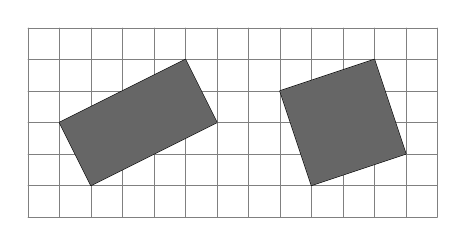
\begin{tikzpicture}[line join=round, line cap=round, >=stealth,font=\footnotesize, scale=0.8]%Hinh nón
	\tikzset{every node/.style={scale=0.7}}% thu nhỏ phóng tỏ tex trong hình
	\draw[style=help lines,step=0.5] (0,0) grid (6.5,3);
	\draw (1,0.5) -- (3,1.5) -- (2.5,2.5)--(0.5,1.5) -- cycle;
	\fill[black!60] (1,0.5) -- (3,1.5) -- (2.5,2.5)--(0.5,1.5);
	\draw (4,2) -- (4.5,0.5) -- (6,1)--(5.5,2.5) -- cycle;
	\fill[black!60] (4,2) -- (4.5,0.5) -- (6,1)--(5.5,2.5);	
	\end{tikzpicture}
}
	\loigiai{
	\begin{center}
	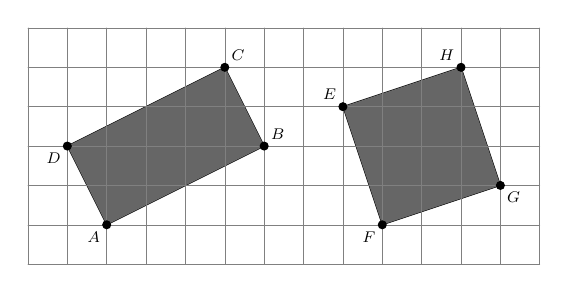
\begin{tikzpicture}[line join=round, line cap=round, >=stealth,font=\footnotesize, scale=1]%Hinh nón
	\tikzset{every node/.style={scale=0.7}}% thu nhỏ phóng tỏ tex trong hình
	\draw (1,0.5) -- (3,1.5) -- (2.5,2.5)--(0.5,1.5) -- cycle;
	\fill[black!60] (1,0.5) -- (3,1.5) -- (2.5,2.5)--(0.5,1.5);
	%	\draw (1.3,1.5) node {e)};
	\draw (4,2) -- (4.5,0.5) -- (6,1)--(5.5,2.5) -- cycle;
	\fill[black!60] (4,2) -- (4.5,0.5) -- (6,1)--(5.5,2.5);
	%	\draw (4,1.2) node {g)};	
	\draw[style=help lines,step=0.5] (0,0) grid (6.5,3);
	\draw[fill=black] 
	(1,0.5) circle (0.05) node[below left] {$A$}	
	(3,1.5) circle (0.05) node[above right] {$B$}
	(2.5,2.5)circle (0.05) node[above right] {$C$}
	(0.5,1.5) circle (0.05) node[below left] {$D$} 
	(4,2) circle (0.05) node[above left] {$E$}	
	(4.5,0.5) circle (0.05) node[below left] {$F$}
	(6,1) circle (0.05) node[below right] {$G$}
	(5.5,2.5) circle (0.05) node[above left] {$H$} 
	;	
	\end{tikzpicture}
	\end{center}
	Gọi hình chữ nhật và hình vuông lần lượt là $ABCD$, $EFGH$. Từ hình vẽ ta có\\
	$$AB=\sqrt{2^2+4^2}=\sqrt{20}; BC=\sqrt{1^2+2^2}=\sqrt{5}.$$ 
	Diện tích hình chữ nhật $ABCD$ là $S_{ABCD}=\sqrt{20} \cdot \sqrt{5} =\sqrt{20 \cdot 5} =10$.\\
	$$EF=\sqrt{1^2+3^2}=\sqrt{10}.$$
	Diện tích hình vuông $EFGH$ là $S_{EFGH}=EF^2 =\sqrt{10}^2 =10$.\\
	Vậy diện tích của hai hình đã cho bằng nhau.
	}
\end{vd}
%%==========Ví dụ 38
\begin{vd}%Vận dụng 2. 
	Biết rằng hình tam giác và hình chữ nhật ở hình sau có diện tích bằng nhau. Tính chiều rộng $x$ của hình chữ nhật.
	\begin{center}
	\begin{tikzpicture}[line join=round, line cap=round, >=stealth,font=\footnotesize, scale=0.8]%Hinh nón
	\tikzset{every node/.style={scale=0.7}}% thu nhỏ phóng tỏ tex trong hình
	set up coordinates for an easy use
	\coordinate (A) at (0,0);
	\coordinate (B) at (5,0);
	\coordinate (C) at (1.5,4);
	\coordinate (H) at ($(B)!(C)!(A)$);
	\draw[<->] ([yshift=-0.15cm]A) -- ([yshift=-0.15cm]B) node[midway, below]{$\sqrt{32}$ cm};
	\coordinate (M) at ($(C)!0.5!(H)$);
	\draw 
	(A)--(B)--(C)--(A) (C)--(H)
	;	
	%	
	\draw[fill=black] 
	(M) node[right] {$\sqrt{27}$ cm}
	;	
	\draw pic[draw,angle radius=2mm] {right angle = A--H--C};	
	\end{tikzpicture} \, \, \, \,
	\begin{tikzpicture}[line join=round, line cap=round, >=stealth,font=\footnotesize, scale=0.8]%Hinh nón
	\tikzset{every node/.style={scale=0.7}}% thu nhỏ phóng tỏ tex trong hình
	set up coordinates for an easy use
	\coordinate (A) at (0,0);
	\coordinate (B) at (5,0);
	\coordinate (C) at (5,3);
	\coordinate (D) at (0,3);
	\coordinate (H) at ($(B)!(A)!(C)$);
	\coordinate (M) at ($(A)!0.5!(B)$);
	\coordinate (N) at ($(C)!0.5!(B)$);
	\draw 
	(A)--(B)--(C)--(D)--(A) 
	;	
	%	
	\draw[fill=black] 
	(M) node[below] {$\sqrt{24}$ cm}
	(N) node[right] {$x$ cm};
	\end{tikzpicture}
	\end{center}
	\loigiai{
	Diện tích tam giác là $\dfrac{1}{2}\cdot \sqrt{32} \cdot \sqrt{27} =\dfrac{1}{2}\cdot 4\sqrt{2}\cdot 3\cdot \sqrt{3} =6\sqrt{2\cdot 3}=6\sqrt{6}$ (cm$^2$).\\
	Diện tích hình chữ nhật là $x\sqrt{24}$ (cm$^2$).\\
	Theo bài ra ta có 
	\[
	\begin{aligned}
	& x\sqrt{24} = 6\sqrt{6} \\
	& x = \dfrac{6\sqrt{6}}{\sqrt{24}} \\
	& x = \dfrac{6\sqrt{6}}{2\sqrt{6}} \\
	& x =3. 
	\end{aligned}
	\]
	Vậy chiều rộng của hình chữ nhật là $3$ (cm).
	}
\end{vd}
%%==========Ví dụ 39
\begin{vd}
	\immini{Bạn Lan cắt một hình chữ nhật $A B C D$ thành những hình tam giác như hình bên (đơn vị tính theo centimét).
	\begin{enumerate}
	\item Tính độ dài các cạnh của hình chữ nhật $A B C D$.
	\item Sau đó, bạn Lan muốn cắt một hình vuông có diện tích bằng diện tích hình chữ nhật $A B C D$. Tính độ dài cạnh của hình vuông đó.
	\end{enumerate}}{\begin{tikzpicture}[scale=1, font=\footnotesize, line join=round, line cap=round, >=stealth]
	\path
	(0,0) coordinate (K)
	(3,0) coordinate (D)
	(0,-3) coordinate (C)
	($(K)!0.5!(D)$) coordinate (M)
	($(K)!0.5!(C)$) coordinate (I)
	($(M)!1!90:(D)$) coordinate (A)
	($(A)!2!(K)$) coordinate (B)
	;
	\draw 
	(A)--(B)--(C)--(D)--(A)--(M)node[midway,right]{$1$} (D)--(M)node[midway,above]{$1$}--(K)node[midway,above]{$1$}--(I)node[midway,left]{$1$}--(C)node[midway,left]{$1$} (B)--(I)node[midway,above]{$1$}
	;
	\foreach \p/\g in {A/90, B/180, C/-90, D/0, M/-90, I/0, K/120}
	\draw[fill=black] (\p) circle (1pt) node[shift=(\g:3mm)] {$\p$};
	\pic[draw,angle radius=2mm]{right angle=A--M--D};
	\pic[draw,angle radius=2mm]{right angle=D--K--C};
	\pic[draw,angle radius=2mm]{right angle=B--I--C};
	\end{tikzpicture}}
	\loigiai{
	\begin{enumerate}
	\item Trong tam giác vuông cân $B I C$, ta có:
	$$
	B C^2=B I^2+C I^2 \text { (theo định lí Pythagore). }
	$$
	Suy ra $B C^2=1^2+1^2=2$. Do đó $B C=\sqrt{2}~\mathrm{cm}$.\\
	Ta có $C K=1+1=2~(\mathrm{cm}); D K=1+1=2~\mathrm{cm}$.\\
	Trong tam giác vuông cân $C K D$, ta có $C D^2=C K^2+D K^2$ (theo định lí Pythagore).\\
	Suy ra $C D^2=2^2+2^2=8$. Do đó $C D=\sqrt{8}~\mathrm{cm}$.\\
	Vậy hình chữ nhật $A B C D$ có $A D=B C=\sqrt{2} ~\mathrm{cm}$, $AB=CD=\sqrt{8}~ \mathrm{cm}$.
	\item Diện tích của hình chữ nhật $A B C D$ là
	$$BC\cdot C D=\sqrt{2} \cdot \sqrt{8}=\sqrt{2 \cdot 8}=\sqrt{16}=4~\mathrm{cm}^2.$$
	Gọi độ dài cạnh của hình vuông là $x~(\mathrm{cm})$ với $x>0$.\\
	Ta có $x^2=4$. Do $x>0$ nên $x=\sqrt{4}$ hay $x=2$.\\
	Vậy độ dài cạnh của hình vuông là $2 ~\mathrm{cm}$.
	\end{enumerate}
	}
\end{vd}
%%%%%%%%%%%%%%%%
\subsection{Bài tập vận dụng}
%%==========Bài 7
\begin{bt}
	Tính:
	\begin{listEX}[4]
	\item $\sqrt{5{,}1^2}$;
	\item $\sqrt{\left(-4{,}9\right)^2}$;
	\item $-\sqrt{\left(-0{,}001\right)^2}$;
	\item $\sqrt{(-10)^{2}}$.
	\end{listEX}
	\loigiai
	{
	\begin{enumerate}
	\item $\sqrt{5{,}1^2}=\big|5{,}1\big|=5{,}1$.
	\item $\sqrt{\left(-4{,}9\right)^2}=\sqrt{\left(4{,}9\right)^2}=\big|4{,}9\big|=4{,}9$.
	\item $-\sqrt{\left(-0{,}001\right)^2}=-\sqrt{\left(0{,}001\right)^2}=-\big|0{,}001\big|=0{,}001$.
	\item $\sqrt{(-10)^{2}}=|-10| =10$.
	\end{enumerate}	
	}
\end{bt}
%%==========Bài 8
\begin{bt}
	Tính:
	\begin{enumEX}{4}
	\item $\sqrt{(-0{,}4)^{2}}$;
	\item $-\sqrt{\left(-\dfrac{4}{9}\right)^{2}}$;
	\item $\sqrt{\left(-\dfrac{2}{7}\right)^{2}}$;
	\item $-2 \sqrt{3^{2}}+(-\sqrt{6})^{2}$.
	\end{enumEX}
	\loigiai{
	\begin{enumEX}{1}
	\item $\sqrt{(-0{,}4)^{2}}=|-0{,}4|=0{,}4$.
	\item $-\sqrt{\left(-\dfrac{4}{9}\right)^{2}}=-\left|-\dfrac{4}{9}\right|=-\dfrac{4}{9}$.
	\item $\sqrt{\left(-\dfrac{2}{7}\right)^{2}}=\left|-\dfrac{2}{7}\right|=\dfrac{2}{7}$.
	\item $-2 \sqrt{3^{2}}+(-\sqrt{6})^{2}=-2\cdot |3|+6=-6+6 =0$.
	\end{enumEX}
	}
\end{bt}
%%==========Bài 32
\begin{bt}
	Rút gọn các biểu thức sau:
	\begin{listEX}[3]
	\item $\sqrt{\left(2-\sqrt{5}\right)^2}$;
	\item $3 \sqrt{x^2}-x+1 \quad(x<0)$;
	\item $\sqrt{x^2-4 x+4} \quad(x<2)$.
	\end{listEX}
	\loigiai
	{
	\begin{enumerate}
	\item $\sqrt{\left(2-\sqrt{5}\right)^2}=\big|2-\sqrt{5}\big|=\sqrt{5}-2$.
	\item $3 \sqrt{x^2}-x+1=3\big|x\big|-x+1=-3x-x+1=-4x+1$. (vì $x<0$)
	\item $\sqrt{x^2-4 x+4}=\sqrt{\left(x-2\right)^2}=\big|x-2\big|=2-x$. (vì $x<2$)
	\end{enumerate}	
	}
\end{bt}
%%==========Bài 33
\begin{bt} 
	Rút gọn các biểu thức sau:
	\begin{enumEX}{3}
	\item $\sqrt{(3-\sqrt{10})^{2}}$;
	\item $2 \sqrt{a^{2}}+4 a$ với $a>0$;
	\item $\sqrt{a^{2}}+\sqrt{(3-a)^{2}}$ với $0<a<3$.
	\end{enumEX}
	\loigiai{
	\begin{enumEX}{1}
	\item $\sqrt{(3-\sqrt{10})^{2}} = |3-\sqrt{10}| = \sqrt{10}-3$ (vì $3-\sqrt{10}<0$).
	\item $2 \sqrt{a^{2}}+4 a=2|a|+4a = 2a+4a=6a$ (vì $a>0$).
	\item $\sqrt{a^{2}}+\sqrt{(3-a)^{2}} = |a| + |3-a| = a+3-a = 3$ (vì $0<a<3$).	
	\end{enumEX}
	}
\end{bt}
%%==========Bài 34
\begin{bt}%[9D1B2]
	Rút gọn các biểu thức sau:
	\begin{listEX}[3]
	\item $\sqrt{\left(3-\sqrt{10}\right)^2}$;
	\item $\sqrt{9-4\sqrt{5}}$;
	\item $3x-\sqrt{x^2-2x+1}$.
	\end{listEX}
	\loigiai
	{
	\begin{listEX}[3]
	\item $\sqrt{10}-3$;
	\item $\sqrt{5}-2$;
	\item $\hoac{&2x+1\;\text{nếu}\; x\geq 1\\&4x-1\;\text{nếu}\;x<1.}$
	\end{listEX}	}
\end{bt}
%%==========Bài 9
\begin{bt} %Thực hành 2. 
	Rút gọn các biểu thức sau:
	\begin{enumEX}{2}
	\item $\sqrt{(2-\sqrt{5})^{2}}$;
	\item $\sqrt{a^{2}}+\sqrt{(-3 a)^{2}}$ với $a>0$.
	\end{enumEX}
	\loigiai{
	\begin{enumEX}{1}
	\item $\sqrt{(2-\sqrt{5})^{2}}=|2-\sqrt{5}|=\sqrt{5}-2$ (vì $2-\sqrt{5}<0$);
	\item $\sqrt{a^{2}}+\sqrt{(-3 a)^{2}}=|a|+|-3a|=|a|+3|a|=4|a|=4a$ (vì $a>0$).
	\end{enumEX}
	}
\end{bt}
%%==========Bài 28
\begin{bt}
	Không dùng $\mathrm{MTCT}$, chứng tỏ biểu thức $A$ có giá trị là số nguyên:
	$$A=\sqrt{\left(1+2\sqrt{2}\right)^2}-\sqrt{\left(1-2\sqrt{2}\right)^2}.$$
	\loigiai
	{
	Ta có \allowdisplaybreaks
	\begin{eqnarray*}
	A&=&\sqrt{\left(1+2\sqrt{2}\right)^2}-\sqrt{\left(1-2\sqrt{2}\right)^2}\\
	&=&\big|1+2\sqrt{2}\big|-\big|1-2\sqrt{2}\big|\\
	&=& 1+2\sqrt{2}+1-2\sqrt{2}\\
	&=& 2.
	\end{eqnarray*}
	Vậy biểu thức $A$ có giá trị nguyên.	
	}
\end{bt}
%%==========Bài 13
\begin{bt}%[9D1B2]
	Tìm $x$ biết
	\begin{listEX}[3]
	\item $\sqrt{x^2-10x+25}=2$;
	\item $\sqrt{x^2}=3x-2$;
	\item $\sqrt{4x^2-12x+9}=x+7$.
	\end{listEX}
	\loigiai
	{
	\begin{listEX}[3]
	\item $x=3$ hoặc $x=7$;
	\item $x=1$;
	\item $x\in\left\lbrace 10;-\dfrac{4}{3}\right\rbrace$.
	\end{listEX}	}
\end{bt}
%%==========Ví dụ 27
\begin{bt}%[9D1K2]
	Tìm $x$, biết $\sqrt{x^2 - 6x + 9} + 7x = 13$.
	\loigiai{
	Ta có 
	$\begin{aligned}[t]
	\sqrt{x^2 - 6x + 9} + 7x &= 13\\
	\sqrt{(x - 3)^2} + 7x &= 13\\
	| x - 3 | + 7x &= 13.
	\end{aligned}$\\
	Nếu $x\geq 3$ thì phương trình trở thành $x - 3 + 7x = 13\Rightarrow 8x = 16\Rightarrow x = 2$ (không thuộc khoảng đang xét).\\
	Nếu $x<3$ thì phương trình trở thành $3 - x + 7x = 13\Rightarrow 6x = 10\Rightarrow x =\dfrac{5}{3}$ (thuộc khoảng đang xét).\\
	Vậy giá trị của $x$ thỏa mãn đẳng thức đã cho là $x=\dfrac{5}{3}$.
	}
\end{bt}
%%==========Bài 1
\begin{bt} 
	Tính:
	\begin{enumEX}{4}
	\item $\sqrt{16 \cdot 0{,}25}$;
	\item $\sqrt{2^{4} \cdot(-7)^{2}}$;
	\item $\sqrt{0{,}9} \cdot \sqrt{ 1000}$;
	\item $\sqrt{2} \cdot \sqrt{5} \cdot \sqrt{40}$.
	\end{enumEX}
	\loigiai{
	\begin{enumEX}{1}
	\item $\sqrt{16 \cdot 0{,}25} = \sqrt{16} \cdot \sqrt{0{,}25} = 4 \cdot 0{,}5=2$.
	\item $\sqrt{2^{4} \cdot(-7)^{2}} = \sqrt{2^{4}} \cdot \sqrt{(-7)^{2}} = 2^2\cdot |-7| = 4\cdot 7 = 28$.
	\item $\sqrt{0,9} \cdot \sqrt{1000}=\sqrt{0{,}9 \cdot 1000} = \sqrt{900} = 30 $.
	\item $\sqrt{2} \cdot \sqrt{5} \cdot \sqrt{40} = \sqrt{2 \cdot 5 \cdot 40} = \sqrt{400} = 20$.	
	\end{enumEX}
	}
\end{bt}
%%==========Bài 2
\begin{bt}
	Rút gọn biểu thức:
	\begin{listEX}[3]
	\item $\sqrt{4a^2}$;
	\item $\sqrt{2a}\cdot\sqrt{8a}$ với $a>0$;
	\item $\sqrt{\dfrac{4a^2}{25}}$.
	\end{listEX}
	\loigiai{
	\begin{enumerate}
	\item $\sqrt{4a^2}=\sqrt{4}\cdot\sqrt{a^2}=2|a|$.
	\item $\sqrt{2a}\cdot\sqrt{8a}=\sqrt{2a\cdot 8a}=\sqrt{16a^2}=\sqrt{16}\cdot\sqrt{a^2}=4|a|=4a$ (vì $a>0)$.
	\item $\sqrt{\dfrac{4 a^2}{25}}=\dfrac{\sqrt{4 a^2}}{\sqrt{25}}=\dfrac{\sqrt{4} \cdot \sqrt{a^2}}{5}=\dfrac{2|a|}{5}$.
	\end{enumerate}
	}
\end{bt}
%%==========Bài 3
\begin{bt}
	Tính
	\begin{listEX}[3]
	\item $\sqrt{12} \cdot(\sqrt{12}+\sqrt{3})$.
	\item $\sqrt{8} \cdot(\sqrt{50}-\sqrt{2})$.
	\item $(\sqrt{3}+\sqrt{2})^2-2 \sqrt{6}$.	
	\end{listEX}
	\loigiai{
	\begin{listEX}[1]
	\item $\sqrt{12} \cdot(\sqrt{12}+\sqrt{3}) = \sqrt{12^2} + \sqrt{36}= \sqrt{12^2} + \sqrt{6^2} = 12 + 6 = 18.$
	\item $\sqrt{8} \cdot(\sqrt{50}-\sqrt{2}) = \sqrt{400} + \sqrt{16} = \sqrt{20^2} + \sqrt{4^2} = 20 + 4 = 24.$
	\item $(\sqrt{3}+\sqrt{2})^2-2 \sqrt{6} = 3+2 + 2\sqrt{6} - 2\sqrt{6} = 5.$
	\end{listEX}
	}
\end{bt}
%%==========Bài 4
\begin{bt}
	So sánh:
	\begin{multicols}{3}
	\begin{enumerate}
	\item $\sqrt{3} \cdot \sqrt{7}$ và $\sqrt{22}$;
	\item $\dfrac{\sqrt{52}}{\sqrt{2}}$ và $5$;
	\item $3 \sqrt{7}$ và $\sqrt{65}$.
	\end{enumerate}
	\end{multicols}
	\loigiai{
	\begin{enumerate}
	\item $\sqrt{3} \cdot \sqrt{7}=\sqrt{3\cdot7}=\sqrt{21} < \sqrt{22}$;
	\item $\dfrac{\sqrt{52}}{\sqrt{2}}=\dfrac{\sqrt{26\cdot2}}{\sqrt{2}}=\sqrt{26}> \sqrt{25}$;
	\item $3 \sqrt{7}=\sqrt{9\cdot7}=\sqrt{63}<\sqrt{65}$.
	\end{enumerate}
	}
\end{bt}
%%==========Bài 5
\begin{bt}%[9D1B3]
	Tính 
	\begin{listEX}[2]
	\item $\sqrt{400\cdot 0,81}$; 
	\item $\sqrt{\dfrac{5}{27} \cdot \dfrac{3}{20}}$;
	\item $\sqrt{(-5)^2 \cdot 3^2}$;
	\item $\sqrt{\left(2-\sqrt{5}\right)^2 \cdot \left(2+\sqrt{5}\right)^2}$. 
	\end{listEX}
	\loigiai{
	\begin{listEX}[2]
	\item $\sqrt{400\cdot 0,81}=18$; 
	\item $\sqrt{\dfrac{5}{27} \cdot \dfrac{3}{20}}=\dfrac{1}{6}$;
	\item $\sqrt{(-5)^2 \cdot 3^2}=15$;
	\item $\sqrt{\left(2-\sqrt{5}\right)^2 \cdot \left(2+\sqrt{5}\right)^2}=1$. 
	\end{listEX}
	}
\end{bt}
%%==========Bài 6
\begin{bt} 
	Rút gọn các biểu thức sau:
	\begin{enumEX}{3}
	\item $\sqrt{8^{2} \cdot 5}$
	\item $\sqrt{8 1a^2}$ với $a<0$;
	\item $\sqrt{5 a} \cdot \sqrt{45 a}-3 a$ với $a \geq 0$.
	\end{enumEX}
	\loigiai{
	\begin{enumEX}{1}
	\item $\sqrt{8^{2} \cdot 5} = 8\cdot \sqrt{5}$.
	\item $\sqrt{81 a^{2}} = 81|a| = -81a$ (vì $a<0$).
	\item 
	$\begin{aligned}[t]
	\sqrt{5 a} \cdot \sqrt{45 a}-3 a & = \sqrt{5 a \cdot 45 a}-3a = \sqrt{15^2 \cdot a^2}-3a \\
	&= 15\cdot |a| -3a = 15a-3a=12a \, (\text {vì } a \geq 0).
	\end{aligned}$
	\end{enumEX}
	}
\end{bt}
%%==========Bài 7
\begin{bt}%[9D1B3]
	Tính
	\begin{listEX}[2]
	\item $\left(\sqrt{x}-3\right) \left(\sqrt{x}+2\right)$; 
	\item $\left(\sqrt{x}-\sqrt{y}\right)\left(\sqrt{x}+\sqrt{y}\right)$;
	\item $\left(\sqrt{\dfrac{25}{3}}-\sqrt{\dfrac{49}{3}}+\sqrt{3}\right) \sqrt{3}$;
	\item $\left(1+\sqrt{3}-\sqrt{5}\right) \left(1+\sqrt{3}+\sqrt{5}\right)$. 
	\end{listEX}
	\loigiai{
	\begin{listEX}[2]
	\item $\left(\sqrt{x}-3\right) \left(\sqrt{x}+2\right) =x-\sqrt{x}-6$; 
	\item $\left(\sqrt{x}-\sqrt{y}\right)\left(\sqrt{x}+\sqrt{y}\right)=x-y$;
	\item $\left(\sqrt{\dfrac{25}{3}}-\sqrt{\dfrac{49}{3}}+\sqrt{3}\right) \sqrt{3}=1$;
	\item $\left(1+\sqrt{3}-\sqrt{5}\right) \left(1+\sqrt{3}+\sqrt{5}\right)=2\sqrt{3}-1$. 
	\end{listEX}	
	}
\end{bt}
%%==========Bài 8
\begin{bt}
	Rút gọn biểu thức $\sqrt{2\left(a^2-b^2\right)} \cdot \sqrt{\dfrac{3}{a+b}}$ (với $a \geq b>0$).	
	\loigiai{
	Với $a \ge b > 0$ ta có
	\begin{eqnarray*}
	&&\sqrt{2\left(a^2-b^2\right)} \cdot \sqrt{\dfrac{3}{a+b}}\\	
	&=&\sqrt{2(a+b)(a-b)} \cdot \sqrt{\dfrac{3}{a+b}}\\
	&=&\sqrt{2}\cdot \sqrt{a+b} \cdot \sqrt{a-b}\cdot \dfrac{\sqrt{3}}{\sqrt{a+b}}\\
	&=&\sqrt{6} \cdot \sqrt{a-b}.
	\end{eqnarray*}	
	}
\end{bt}
%%==========Bài 9
\begin{bt}
	Áp dụng quy tắc về căn thức bậc hai của một tích, hãy rút gọn biểu thức:
	\begin{enumEX}{2}
	\item $\sqrt{25(a+1)^2}$ với $a>-1$;
	\item $\sqrt{x^2(x-5)^2}$ với $x>5$;
	\item $\sqrt{2 b} \cdot \sqrt{32 b}$ với $b>0$;
	\item $\sqrt{3 c} \cdot \sqrt{27 c^3}$ với $c>0$.	
	\end{enumEX}
	\loigiai{
	\begin{enumerate}
	\item $\sqrt{25(a+1)^2}=\sqrt{25}\cdot \sqrt{(a+1)^2}=5\cdot |a+1|=5a+5$ (vì $a>-1$ nên $a+1>0$).
	\item $\sqrt{x^2(x-5)^2}=\sqrt{x^2}\cdot \sqrt{(x-5)^2}=x\cdot(x-5)=x^2-5x$ (vì $x>5$ nên $x-5>0$).
	\item $\sqrt{2 b} \cdot \sqrt{32 b}=\sqrt{2b\cdot 32b}=\sqrt{64b^2}=\sqrt{64}\cdot \sqrt{b^2}=8\cdot |b|=8b$ (vì $b>0$).
	\item $\sqrt{3 c} \cdot \sqrt{27 c^3}=\sqrt{3c\cdot 27c^3}=\sqrt{81c^4}=\sqrt{81}\cdot \sqrt{c^4}=9\cdot |c^2|=9c^2$ (vì $c^2>0$).	
	\end{enumerate}
	}
\end{bt}
%%==========Bài 10
\begin{bt}
	Tính
	\begin{listEX}[3]
	\item $\sqrt{99}: \sqrt{11}$.
	\item $\sqrt{7{,}84}$.
	\item $\sqrt{1815}: \sqrt{15}$.	
	\end{listEX}
	\loigiai{
	\begin{enumerate}
	\item $\sqrt{99}: \sqrt{11} = \sqrt{99:11} = \sqrt{9} = 3.$
	\item Ta có $7{,}84 = \dfrac{784}{100} = \dfrac{28^2}{10^2}$
	nên
	$\sqrt{7{,}84} = \sqrt{\dfrac{28^2}{10^2}} = \dfrac{28}{10} = 2{,}8.$
	\item $\sqrt{1815}: \sqrt{15} = \sqrt{1815:15} = \sqrt{121} = 11.$
	\end{enumerate}	
	}
\end{bt}
%%==========Bài 11
\begin{bt} 
	Tính
	\begin{enumEX}{4}
	\item $\sqrt{\dfrac{0{,}49}{81}}$;
	\item $\sqrt{2 \dfrac{7}{9}}$;
	\item $\sqrt{\dfrac{1}{16} \cdot \dfrac{9}{36}}$;
	\item $(-\sqrt{52}): \sqrt{13}$.
	\end{enumEX}
	\loigiai{
	\begin{enumEX}{1}
	\item $\sqrt{\dfrac{0{,}49}{81}} = \dfrac{\sqrt{0{,}49}}{\sqrt{81}}=\dfrac{0{,}7}{9}$.
	\item $\sqrt{2 \dfrac{7}{9}} = \sqrt{ \dfrac{25}{9}} = \dfrac{\sqrt{25}}{\sqrt{9}}= \dfrac{5}{3}$.
	\item $\sqrt{\dfrac{1}{16} \cdot \dfrac{9}{36}} =\dfrac{1}{\sqrt{16}} \cdot \dfrac{\sqrt{9}}{\sqrt{36}} =\dfrac{1}{4} \cdot \dfrac{3}{6}=\dfrac{1}{8}$.
	\item $(-\sqrt{52}): \sqrt{13} =- \dfrac{\sqrt{52}}{\sqrt{13}} = -\sqrt{\dfrac{52}{13}}=-\sqrt{4}=-2$.
	\end{enumEX}
	}
\end{bt}
%%==========Bài 12
\begin{bt}
	Áp dụng quy tắc về căn bậc hai của một tích, hãy tính:
	\begin{listEX}[4]
	\item $\sqrt{36 \cdot 81}$;
	\item $\sqrt{49 \cdot 121 \cdot 169}$;
	\item $\sqrt{50^2-14^2}$;
	\item $\sqrt{3+\sqrt{5}} \cdot \sqrt{3-\sqrt{5}}$.
	\end{listEX}
	\loigiai{
	\begin{enumerate}
	\item $\sqrt{36 \cdot 81}=\sqrt{36}\cdot \sqrt{81}=\sqrt{6^2}\cdot \sqrt{9^2}=6\cdot 9=54$.
	\item $\sqrt{49 \cdot 121 \cdot 169}=\sqrt{49}\cdot \sqrt{121}\cdot \sqrt{169}=7\cdot 11\cdot 13=1001$.
	\item $\sqrt{50^2-14^2}=\sqrt{(50-14)(50+14)}=\sqrt{36\cdot 64}=\sqrt{36}\cdot \sqrt{64}=6\cdot 8=48$.
	\item $\sqrt{3+\sqrt{5}} \cdot \sqrt{3-\sqrt{5}}=\sqrt{\left(3+\sqrt{5}\right)\left(3-\sqrt{5}\right)}=\sqrt{3^2-\left(\sqrt{5}\right)^2}=\sqrt{9-5}=\sqrt{4}=2$.
	\end{enumerate}
	}
\end{bt}
%%==========Bài 13
\begin{bt}
	Áp dụng quy tắc về căn bậc hai của một thương, hãy tính:
	\begin{multicols}{4}
	\begin{enumerate}
	\item $\sqrt{\dfrac{49}{36}}$;
	\item $\sqrt{\dfrac{13^2-12^2}{81}}$;
	\item $\dfrac{\sqrt{9^3+7^3}}{\sqrt{9^2-9 \cdot 7+7^2}}$;
	\item $\dfrac{\sqrt{50^3-1}}{\sqrt{50^2+51}}$.
	\end{enumerate}
	\end{multicols}
	\loigiai{
	\begin{enumerate}
	\item $\sqrt{\dfrac{49}{36}}=\dfrac{7}{6}$;
	\item $\sqrt{\dfrac{13^2-12^2}{81}}=\sqrt{\dfrac{25}{81}}=\dfrac{5}{9}$;
	\item $\dfrac{\sqrt{9^3+7^3}}{\sqrt{9^2-9 \cdot 7+7^2}}=\dfrac{\sqrt{{(9+7)(9^2-9 \cdot 7+7^2)}}}{\sqrt{9^2-9 \cdot 7+7^2}}=\sqrt{9+7}=4$;
	\item $\dfrac{\sqrt{50^3-1}}{\sqrt{50^2+51}}=\dfrac{\sqrt{(50-1)(50^2+50\cdot1+1^2)}}{\sqrt{50^2+50\cdot1+1^2}}=\sqrt{50-1}=7$.	
	\end{enumerate}
	}
\end{bt}
%%==========Bài 14
\begin{bt}%[9D1Y4]
	Tính
	\begin{listEX}[2]
	\item$\sqrt{72}:\sqrt{8}$;
	\item $(\sqrt{28} - \sqrt{7} + \sqrt{112}) :\sqrt{7}$.
	\end{listEX}
	\loigiai
	{
	\begin{listEX}[1]
	\item$\sqrt{72}:\sqrt{8}=\sqrt{\dfrac{72}{8}}=\sqrt{9}=3$.
	\item $(\sqrt{28} - \sqrt{7} + \sqrt{112}) :\sqrt{7}=\sqrt{28}:\sqrt{7} - \sqrt{7}:\sqrt{7} + \sqrt{112}:\sqrt{7}=\sqrt{4}-1+\sqrt{16}=2-1+4=5$.
	\end{listEX}
	}
\end{bt}
%%==========Bài 15
\begin{bt}%[9D1Y4]
	Tính
	\begin{listEX}[3]
	\item $\sqrt{\dfrac{49}{8}}:\sqrt{3\dfrac{1}{8}}$;
	\item $\sqrt{54x}:\sqrt{6x}$;
	\item $\sqrt{\dfrac{1}{125}}\cdot\sqrt{\dfrac{32}{35}}:\sqrt{\dfrac{56}{225}}$.
	\end{listEX}
	\loigiai
	{
	\begin{listEX}[1]
	\item $\sqrt{\dfrac{49}{8}}:\sqrt{3\dfrac{1}{8}}=\sqrt{\dfrac{49}{8}:\dfrac{25}{8}}=\sqrt{\dfrac{49}{25}}=\dfrac{7}{5}$;
	\item $\sqrt{54x}:\sqrt{6x}=\sqrt{\dfrac{54x}{6x}}=\sqrt{9}=3$;
	\item $\sqrt{\dfrac{1}{125}}\cdot\sqrt{\dfrac{32}{35}}:\sqrt{\dfrac{56}{225}}
	=\sqrt{\dfrac{1}{125}\cdot\dfrac{32}{35}:\dfrac{56}{225}}
	=\dfrac{6}{35}$.	
	\end{listEX}
	}
\end{bt}
%%==========Bài 16
\begin{bt}
	Rút gọn $\dfrac{-3 \sqrt{16 a}+5 a \sqrt{16 a b^2}}{2 \sqrt{a}}$ (với $a>0$; $b>0$).	
	\loigiai{
	Với $a >0$; $b>0$ ta có
	\[\dfrac{-3 \sqrt{16 a}+5 a \sqrt{16 a b^2}}{2 \sqrt{a}} = \dfrac{\sqrt{16a} \cdot (-3 + 5a \sqrt{b^2}))}{2\sqrt{a}}=\dfrac{4\sqrt{a} \cdot (-3 + 5ab)}{2\sqrt{a}} =2 \cdot (-3 + 5ab).\]	
	}
\end{bt}
%%==========Bài 17
\begin{bt} 
	Rút gọn các biểu thức sau:
	\begin{enumEX}{2}
	\item $\dfrac{\sqrt{24 a^{3}}}{\sqrt{6 a}}$ với $a>0$;
	\item $\sqrt{\dfrac{3 a^{2} b}{27}}$ với $a \leq 0, b \geq 0$.
	\end{enumEX}
	\loigiai{
	\begin{enumEX}{1}
	\item $\dfrac{\sqrt{24 a^{3}}}{\sqrt{6 a}}=\sqrt{\dfrac{24a^3}{6a}} = \sqrt{4a^2} = 2|a| = 2a$ (vì $a>0$).
	\item $\sqrt{\dfrac{3 a^{2} b}{27}}=\sqrt{\dfrac{ a^{2} b}{9}} = \sqrt{\dfrac{ a^{2}}{9}\cdot b} = \left|\dfrac{a}{3}\right|\cdot \sqrt{b} = \dfrac{-a\sqrt{b}}{3}$ (vì $a \leq 0, b \geq 0$).
	\end{enumEX}
	}
\end{bt}
%%==========Bài 18
\begin{bt}
	Áp dụng quy tắc về căn thức bậc hai của một thương, hãy rút gọn biểu thức:
	\begin{enumEX}{2}
	\item $\sqrt{\dfrac{(3-a)^2}{9}}$ với $a>3$;
	\item $\dfrac{\sqrt{75 x^5}}{\sqrt{5 x^3}}$ với $x>0$;
	\item $\sqrt{\dfrac{9}{x^2-2 x+1}}$ với $x>1$;
	\item $\sqrt{\dfrac{x^2-4 x+4}{x^2+6 x+9}}$ với $x \geq 2$.	
	\end{enumEX}
	\loigiai{
	\begin{enumerate}
	\item $\sqrt{\dfrac{(3-a)^2}{9}}=\dfrac{\sqrt{(3-a)^2}}{\sqrt{9}}=\dfrac{|3-a|}{3}=\dfrac{-(3-a)}{3}=\dfrac{a-3}{3}$ (vì $a>3$ nên $3-a<0$).
	\item $\dfrac{\sqrt{75x^5}}{\sqrt{5 x^3}}=\sqrt{\dfrac{75x^5}{5x^3}}=\sqrt{25x^2}=\sqrt{25}\cdot \sqrt{x^2}=5\cdot |x|=5x$ (vì $x>0$).
	\item $\sqrt{\dfrac{9}{x^2-2 x+1}}=\dfrac{\sqrt{9}}{\sqrt{(x-1)^2}}=\dfrac{3}{|x-1|}=\dfrac{3}{x-1}$ (vì $x>1$ nên $x-1>0$).
	\item $\sqrt{\dfrac{x^2-4 x+4}{x^2+6x+9}}=\dfrac{\sqrt{(x-2)^2}}{\sqrt{(x+3)^2}}=\dfrac{|x-2|}{|x+3|}=\dfrac{x-2}{x+3}$ (vì $x\ge 2$ nên $x-2\geq0$ và $x+3>0$).	
	\end{enumerate}
	}
\end{bt}
%%==========Bài 19
\begin{bt}
Kích thước màn hình ti vi hình chữ nhật được xác định bởi độ dài đường chéo. Một loại ti vi có tỉ lệ hai cạnh màn hình là $4: 3$.
\begin{enumerate}
	\item Gọi $x$ (inch) là chiều rộng của màn hình ti vi. Viết công thức tính độ dài đường chéo $d$ (inch) của màn hình ti vi theo $x$.
	\item Tính chiều rộng và chiều dài (theo centimét) của màn hình ti vi loại $40$ inch.
\end{enumerate}	
\loigiai{
\begin{enumerate}
	\item Chiều dài của màn hình ti vi là $y = \dfrac{4}{3}x$ (inch).\\
	Công thức tính độ dài đường chéo của màn hình ti vi là
	\[d^2 = x^2 + \left( \dfrac{4}{3}x\right) ^2 = x^2 + \dfrac{16}{9}x^2 = \dfrac{25x^2}{9} \Rightarrow d = \dfrac{5}{3}x.\]
	\item Ta có
	\[d = \dfrac{5}{3}x \Rightarrow x = \dfrac{3d}{5}.\]
	Do đó chiều rộng của ti vi loại $40$ inch là
	\[x = \dfrac{3d}{5} = \dfrac{120}{5} = 24\;(\text{inch}).\]
	Chiều dài của ti vi loại $40$ inch là $\dfrac{4}{3}x = \dfrac{4}{3} \cdot 24 = 32\;(\text{inch})$.
\end{enumerate}	
	}
\end{bt}
%%==========Bài 20
\begin{bt} 
	Cho hình chữ nhật có chiều rộng $a$ (cm), chiều dài $b$ (cm) và diện tích $S$ cm$^{2}$.
	\begin{enumEX}{2}
	\item Tìm $S$, biết $a=\sqrt{8}, b=\sqrt{32}$;
	\item Tìm $b$, biết $S=3 \sqrt{2}, a=2 \sqrt{3}$.
	\end{enumEX}
	\loigiai{
	\begin{enumEX}{1}
	\item Ta có $S=ab =\sqrt{8}\cdot \sqrt{32} = \sqrt{8\cdot 32} =16$;
	\item Ta có 
	$$
	\begin{aligned}
	&S=ab \\
	&3 \sqrt{2}=2 \sqrt{3}\cdot b\\
	& b=\dfrac{3 \sqrt{2}}{2 \sqrt{3}} \\
	& b = \sqrt{\dfrac{3^2\cdot 2}{2^2\cdot 3}}\\
	& b = \sqrt{\dfrac{3}{2}}.	 	 
	\end{aligned}	 
	$$
	Vậy $b= \sqrt{\dfrac{3}{2}}$.
	\end{enumEX}
	}
\end{bt}
%%==========Bài 21
\begin{bt} 
	Từ một tấm thép hình vuông, ngươi thợ cắt ta hai mảnh hình vuông có diện tích lần lượt là $24$ cm$^{2}$ và $40$ cm$^{2}$ như hình dưới. Tính diện tích phần còn lại của tấm thép.
	\begin{center}
	\begin{tikzpicture}[line join=round, line cap=round, >=stealth,font=\footnotesize, scale=0.8]%Hinh nón
	\tikzset{every node/.style={scale=0.7}}% thu nhỏ phóng tỏ tex trong hình
	%	\clip(-3.5,-0.5) rectangle (7,6.5);
	set up coordinates for an easy use
	\coordinate (A) at (0,0);
	\coordinate (B) at (5,0);
	\coordinate (C) at (5,5);
	\coordinate (D) at (0,5);
	\coordinate (M) at ($(A)!0.66!(B)$);
	\coordinate (N) at ($(D)!0.66!(C)$);
	\coordinate (P) at ($(A)!0.66!(D)$);
	\coordinate (Q) at ($(B)!0.66!(C)$);
	\coordinate (I) at (intersection of M--N and P--Q);
	\coordinate (x) at (intersection of A--I and P--M);
	\coordinate (y) at (intersection of Q--N and I--C);
	%	\coordinate (H) at ($(B)!(C)!(A)$);
	\draw 
	(A)--(B)--(C)--(D)--(A) (P)--(Q) (M)--(N)
	;	
	\fill[black!60] (P) -- (I) -- (N) -- (D);
	\fill[black!60] (M) -- (B) -- (Q) -- (I);
	%	
	\draw[fill=black] 
	% 	(A) circle (0.05) node[below] {$A$}
	% 	(B) circle (0.05) node[below] {$B$}
	% 	(C) circle (0.05) node[above] {$C$}
	% 	(D) circle (0.05) node[above] {$D$}
	% 	(M) circle (0.05) node[below] {$M$}
	% 	(N) circle (0.05) node[above] {$N$}
	% 	(P) circle (0.05) node[left] {$P$}
	% 	(Q) circle (0.05) node[right] {$Q$}
	% 	(I) circle (0.05) node[below left] {$I$}
	(x) node {$40$ cm$^2$}
	(y) node {$24$ cm$^2$}
	;	
	%	\draw pic[draw,angle radius=2mm] {right angle = A--H--C};
	%	\draw pic[draw,angle radius=2mm] {right angle = O--N--P};
	%	\draw pic[draw,angle radius=2mm] {right angle = M--N--I};	
	%	\draw pic[draw,angle radius=3.5mm] {angle = P--A--C};	
	\path (current bounding box.south) node[below]{\textit{Hình $4$}};% ghi chú hình chuẩn	
	\end{tikzpicture} 	
	\end{center}
	\loigiai{
	\begin{center}
	\begin{tikzpicture}[line join=round, line cap=round, >=stealth,font=\footnotesize, scale=0.8]%Hinh nón
	\tikzset{every node/.style={scale=0.7}}% thu nhỏ phóng tỏ tex trong hình
	%	\clip(-3.5,-0.5) rectangle (7,6.5);
	set up coordinates for an easy use
	\coordinate (A) at (0,0);
	\coordinate (B) at (5,0);
	\coordinate (C) at (5,5);
	\coordinate (D) at (0,5);
	\coordinate (M) at ($(A)!0.66!(B)$);
	\coordinate (N) at ($(D)!0.66!(C)$);
	\coordinate (P) at ($(A)!0.66!(D)$);
	\coordinate (Q) at ($(B)!0.66!(C)$);
	\coordinate (I) at (intersection of M--N and P--Q);
	\coordinate (x) at (intersection of A--I and P--M);
	\coordinate (y) at (intersection of Q--N and I--C);
	%	\coordinate (H) at ($(B)!(C)!(A)$);
	\draw 
	(A)--(B)--(C)--(D)--(A) (P)--(Q) (M)--(N)
	;	
	\fill[black!60] (P) -- (I) -- (N) -- (D);
	\fill[black!60] (M) -- (B) -- (Q) -- (I);
	%	
	\draw[fill=black] 
	(A) circle (0.05) node[below] {$A$}
	(B) circle (0.05) node[below] {$B$}
	(C) circle (0.05) node[above] {$C$}
	(D) circle (0.05) node[above] {$D$}
	(M) circle (0.05) node[below] {$M$}
	(N) circle (0.05) node[above] {$N$}
	(P) circle (0.05) node[left] {$P$}
	(Q) circle (0.05) node[right] {$Q$}
	(I) circle (0.05) node[below left] {$I$}
	(x) node {$40$ cm$^2$}
	(y) node {$24$ cm$^2$}
	;	
	%	\draw pic[draw,angle radius=2mm] {right angle = A--H--C};
	%	\draw pic[draw,angle radius=2mm] {right angle = O--N--P};
	%	\draw pic[draw,angle radius=2mm] {right angle = M--N--I};	
	%	\draw pic[draw,angle radius=3.5mm] {angle = P--A--C};	
	%	\path (current bounding box.south) node[below]{\textit{Hình $4$}};% ghi chú hình chuẩn	
	\end{tikzpicture} 	
	\end{center}
	Ta gán các đỉnh $A$, $B$, $C$, $D$, $P$, $Q$, $M$, $N$, $I$ như hình vẽ. \\
	$S_{AMIP} = IP^2$ suy ra $IP^2=40$ hay $IP = \sqrt{40}$.\\
	$S_{IQCN} = IN^2$ suy ra $IN^2=24$ hay $IN = \sqrt{24}$.\\
	$S_{PIND}=S_{IQBM}=PI\cdot IN = \sqrt{40} \cdot \sqrt{24} = \sqrt{40\cdot 24} = 8\sqrt{15}$.\\
	Vậy diện tích phần còn lại là $2S_{PIND}=16\sqrt{15}$.
	}
\end{bt}
%%==========Bài 22
\begin{bt}
	Cho tam giác đều $ABC$ có độ dài cạnh là $a$. Tính độ dài đường cao $AH$ của tam giác $ABC$ theo $a$.
	\loigiai{
	\begin{center}
	\begin{tikzpicture}[scale=0.8, font=\footnotesize,line join=round, line cap=round, >=stealth]
	\def\canh{4}
	\coordinate (B) at (0,0);
	\coordinate (C) at (\canh,0);
	\coordinate (A) at ($(B) + (60:\canh)$);
	\coordinate (H) at ($(B)!0.5!(C)$);
	\draw(A)--(B)--(C)--cycle;
	\draw(A)--(H);
	\pic[draw,thin,angle radius=2mm] {right angle = A--H--C};
	\path (A)--(B) node[midway,sloped,scale=0.5]{$|$};
	\path (A)--(C) node[midway,sloped,scale=0.5]{$|$};
	\path (B)--(C) node[midway,sloped,scale=0.5]{$|$};
	\foreach \i/\g in {A/90,B/-90,C/-90,H/-90}{\draw[fill=black](\i) circle (1.5pt) ($(\i)+(\g:3mm)$) node[scale=1]{$\i$};}
	\end{tikzpicture}
	\end{center}
	Ta có tam giác $ABC$ đều cạnh $a$, gọi $H$ là trung điểm cạnh $BC$ suy ra $AH$ vuông góc với $BC$ và $BC=\dfrac{a}{2}$.\\
	Xét tam giác vuông $AHC$, áp dụng dịnh lý py-ta-go ta có: 
	$$AH=\sqrt{AC^2 - MC^2} = \sqrt{a^2 - \left(\dfrac{a}{2}\right)^2}=\sqrt{\dfrac{3a^2}{4}}=\dfrac{a\sqrt{3}}{2}.$$
	Vậy đường cao $AH=\dfrac{a\sqrt{3}}{2}$.
	}
\end{bt}
%%==========Bài 23
\begin{bt}
	Trong Vật lí, ta có định luật Joule - Lenz để tính nhiệt lượng toả ra ở dây dẫn khi có dòng điện chạy qua:
	$$Q=I^2 R t$$
	Trong đó:
	\begin{itemize}
	\item $Q$ là nhiệt lượng toả ra trên dây dẫn tính theo Jun $(\mathrm{J})$;
	\item $I$ là cường độ dòng điện chạy trong dây dẫn tính theo Ampe $(\mathrm{A})$;
	\item $R$ là điện trở dây dẫn tính theo $\mathrm{Ohm}(\Omega)$;
	\item $t$ là thời gian dòng điện chạy qua dây dẫn tính theo giây.
	\end{itemize}
	\hspace{0.5 cm} Áp dụng công thức trên để giải bài toán sau: Một bếp điện khi hoạt động bình thường có điện trở $R=80 \,\Omega$. Tính cường độ dòng điện chạy trong dây dẫn, biết nhiệt lượng mà dây dẫn toả ra trong 1 giây là $500 \mathrm{~J}$.	
	\loigiai{
	Áp dụng công thức $Q=I^2 R t$, cường độ dòng điện chạy trong dây dẫn: 
	$$I=\sqrt{\dfrac{Q}{Rt}}=\sqrt{\dfrac{500}{80\cdot1}}=\sqrt{\dfrac{25}{4}}=\dfrac{5}{2}.$$
	Vậy cường độ dòng điện chạy trong dây dẫn là $I=\sqrt{\dfrac{Q}{Rt}}=\dfrac{5}{2}.$	
	}
\end{bt}
%%==========Bài 24
\begin{bt}
	Tốc độ gần đúng của một ô-tô ngay trước khi đạp phanh được tính theo công thức $v=\sqrt{2 \lambda g d}$, trong đó $v\,(\mathrm{m} / \mathrm{s})$ là tốc độ của ô-tô, $d\,(\mathrm{m})$ là chiều dài của vết trượt tính từ thời điểm đạp phanh cho đến khi ô tô dừng lại trên đường, $\lambda$ là hệ số cản lăn của mặt đường, $g=9,8 \mathrm{~m} / \mathrm{s}^2$ (Nguồn: $J$. Libby, Math for Real Life: Teaching Practical Uses for Algebra, McFarland, năm 2017). Nếu một chiếc ô-tô để lại vết trượt dài khoảng $20 \mathrm{~m}$ trên đường nhựa thì tốc độ của ô-tô trước khi đạp phanh là khoảng bao nhiêu mét trên giây (làm tròn kết quả đến hàng đơn vị)? Biết rằng hệ số cản lăn của đường nhựa là $\lambda=0{,}7$.
\begin{center}
	\includegraphics[width=0.55\linewidth]{images/9C3-2-1}	\\
	Vết trượt của xe ô-tô 
\end{center}
	\loigiai{
	Tốc độ của ô-tô	trước khi đạp phanh là $$v=\sqrt{2 \lambda g d}=\sqrt{2\cdot 0{,}7\cdot 9{,}8\cdot 20}=\sqrt{\dfrac{2^3\cdot7^3}{10}}=\dfrac{14\sqrt{35}}{5}.$$	
	}
\end{bt}
%%==========Bài 25
\begin{bt}%[9D1K3]
	Phân tích thành nhân tử
	\begin{listEX}[2]
	\item $a-5\sqrt{a}$;
	\item $a-7$ với $a>0$;
	\item $a+4\sqrt{a}+4$;
	\item $\sqrt{xy}-4\sqrt{x}+3\sqrt{y}-12$.
	\end{listEX}
	\loigiai{
	\begin{listEX}[2]
	\item $a-5\sqrt{a}=\sqrt{a}(\sqrt{a}-5)$;
	\item $a-7= \left(\sqrt{a}-\sqrt{7}\right)\left(\sqrt{a}+\sqrt{7}\right)$ ;
	\item $a+4\sqrt{a}+4=\left(\sqrt{a}+2 \right)^2$;
	\item $\sqrt{xy}-4\sqrt{x}+3\sqrt{y}-12=\left(\sqrt{x}+3 \right) \left(\sqrt{y}-4 \right)$.
	\end{listEX}
	}
\end{bt}
%%==========Bài 26
\begin{bt}%[9D1B3]
	Chứng minh rằng $\sqrt{7}-\sqrt{3}<\sqrt{6}-\sqrt{2}$.
	\loigiai{
	Ta có 
	$\begin{aligned}[t]
	&\left(\sqrt{7}+\sqrt{2}\right)^2=9+2 \sqrt{14}\\
	&\left(\sqrt{6}+\sqrt{3}\right)^2=9+2 \sqrt{18}	 
	\end{aligned}$\\
	Vì $9+2 \sqrt{14}<9+2 \sqrt{18}$ nên $\left(\sqrt{7}+\sqrt{2}\right)^2<\left(\sqrt{6}+\sqrt{3}\right)^2$.\\
	Hay $\sqrt{7}-\sqrt{3}<\sqrt{6}-\sqrt{2}$.
	}
\end{bt}
%%==========Bài 27
\begin{bt}%[9D1K3]
	Tìm $x$ biết 
	\begin{listEX}[2]
	\item $\sqrt{49\left(1-2 x+x^2\right)}-35=0$; 
	\item $\sqrt{x^2-9}-5 \sqrt{x+3}=0$.
	\end{listEX}
	\loigiai{
	\begin{listEX}[2]
	\item $x_1=6$; $x_2=-4$;
	\item $x_1=-3$; $x_2=28$.
	\end{listEX}	
	}
\end{bt}
%%==========Bài 28
\begin{bt}%[9D1K3]
	Tính giá trị của biểu thức $A=\sqrt{7+\sqrt{13}}-\sqrt{7-\sqrt{13}}$. 
	\loigiai{
	Hướng dẫn: Tính $A^2=2$, suy ra $A=\sqrt{2}$.
	}
\end{bt}